\section{Results from $bb\tau\tau$}

The postfit final $m_{\tau\tau}$ distributions in the signal region (SR) and control regions (CRs) for 1 and 2 b-tag jet multiplicities, are shown for the $\mu\tau_{h}$ channel in Fig. \ref{fig:results_mtt_postfit_mtall}, $e\tau_{h}$ channel in Fig. \ref{fig:results_mtt_postfit_etall}, and $e\mu$ channel in Fig. \ref{fig:results_mtt_postfit_emall}.
\begin{figure}[ht]
    \begin{center}
        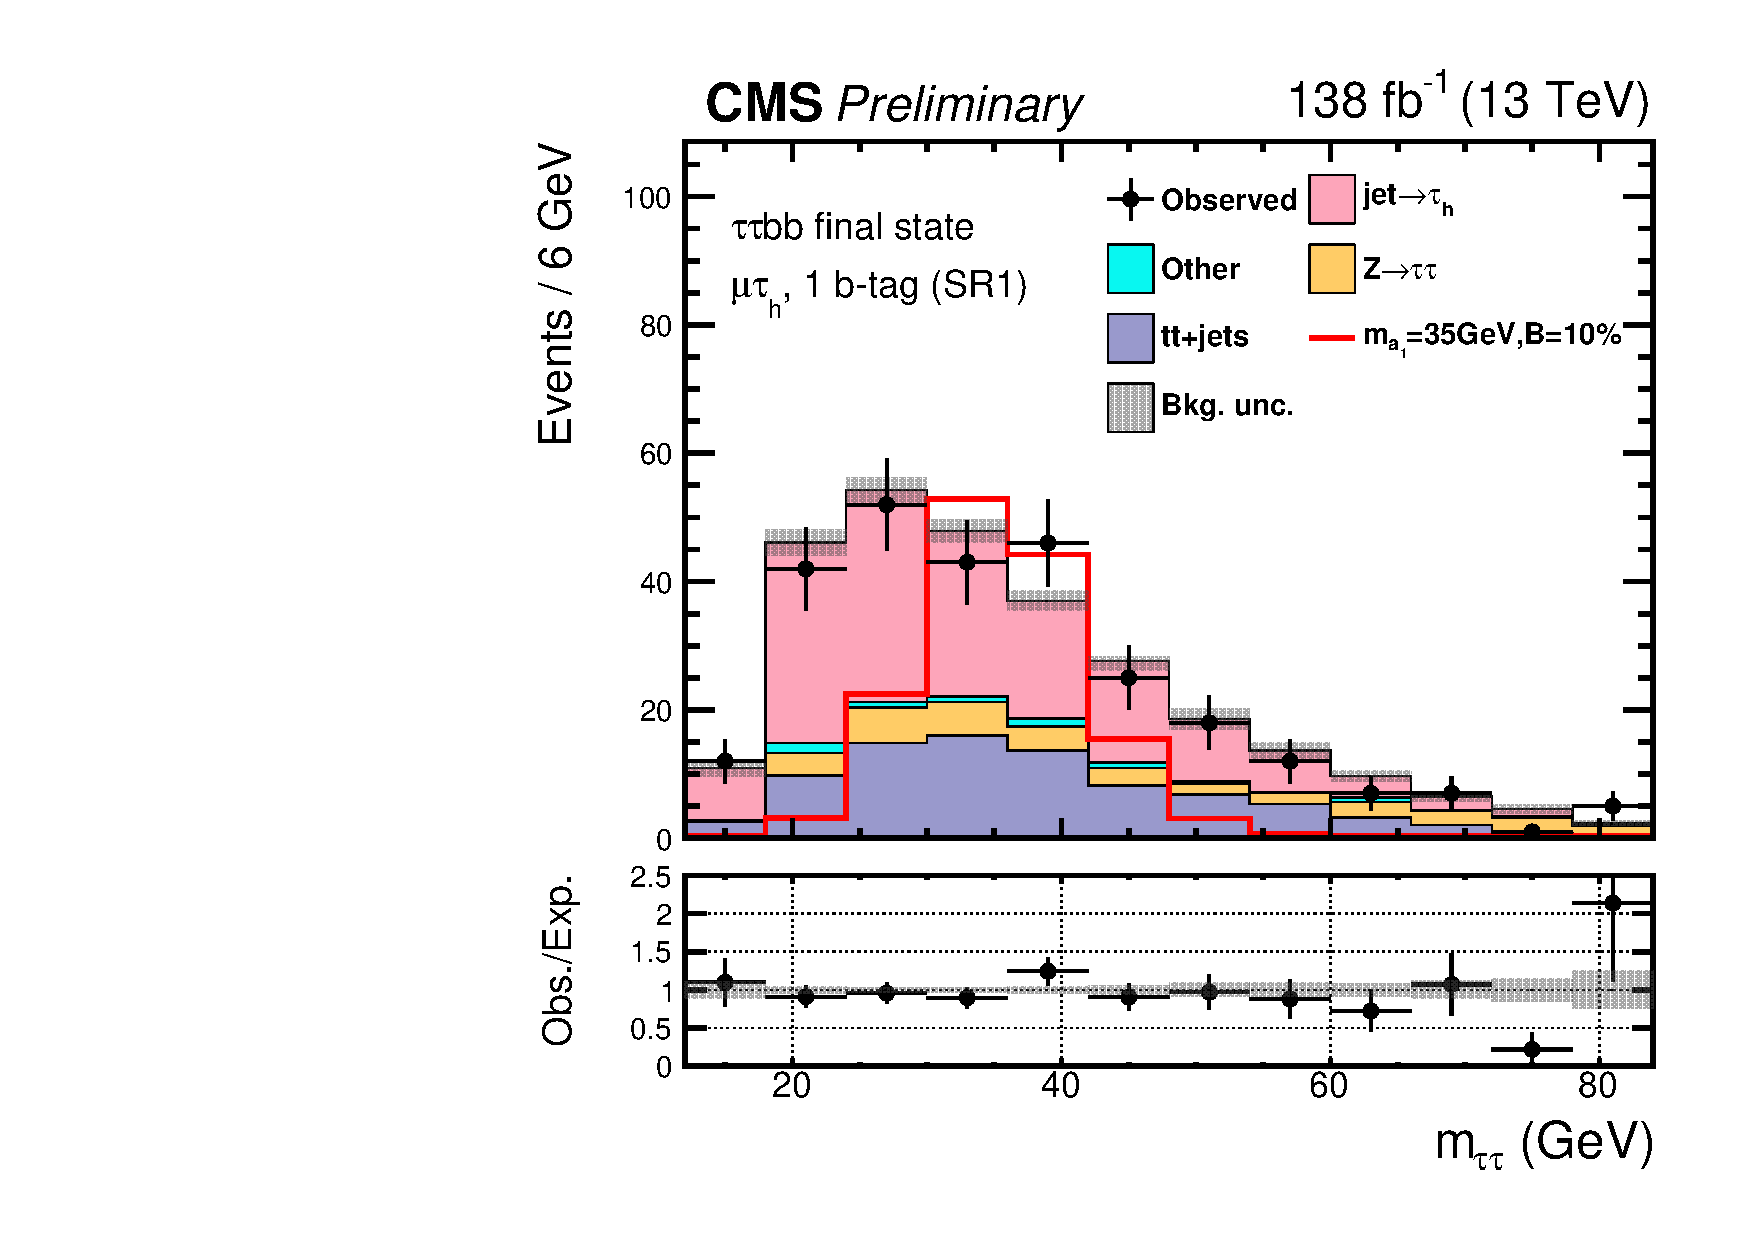
\includegraphics[width=0.32\textwidth]{figures/ch-13-results/mt_all_1_post_prelim-yes.pdf}
        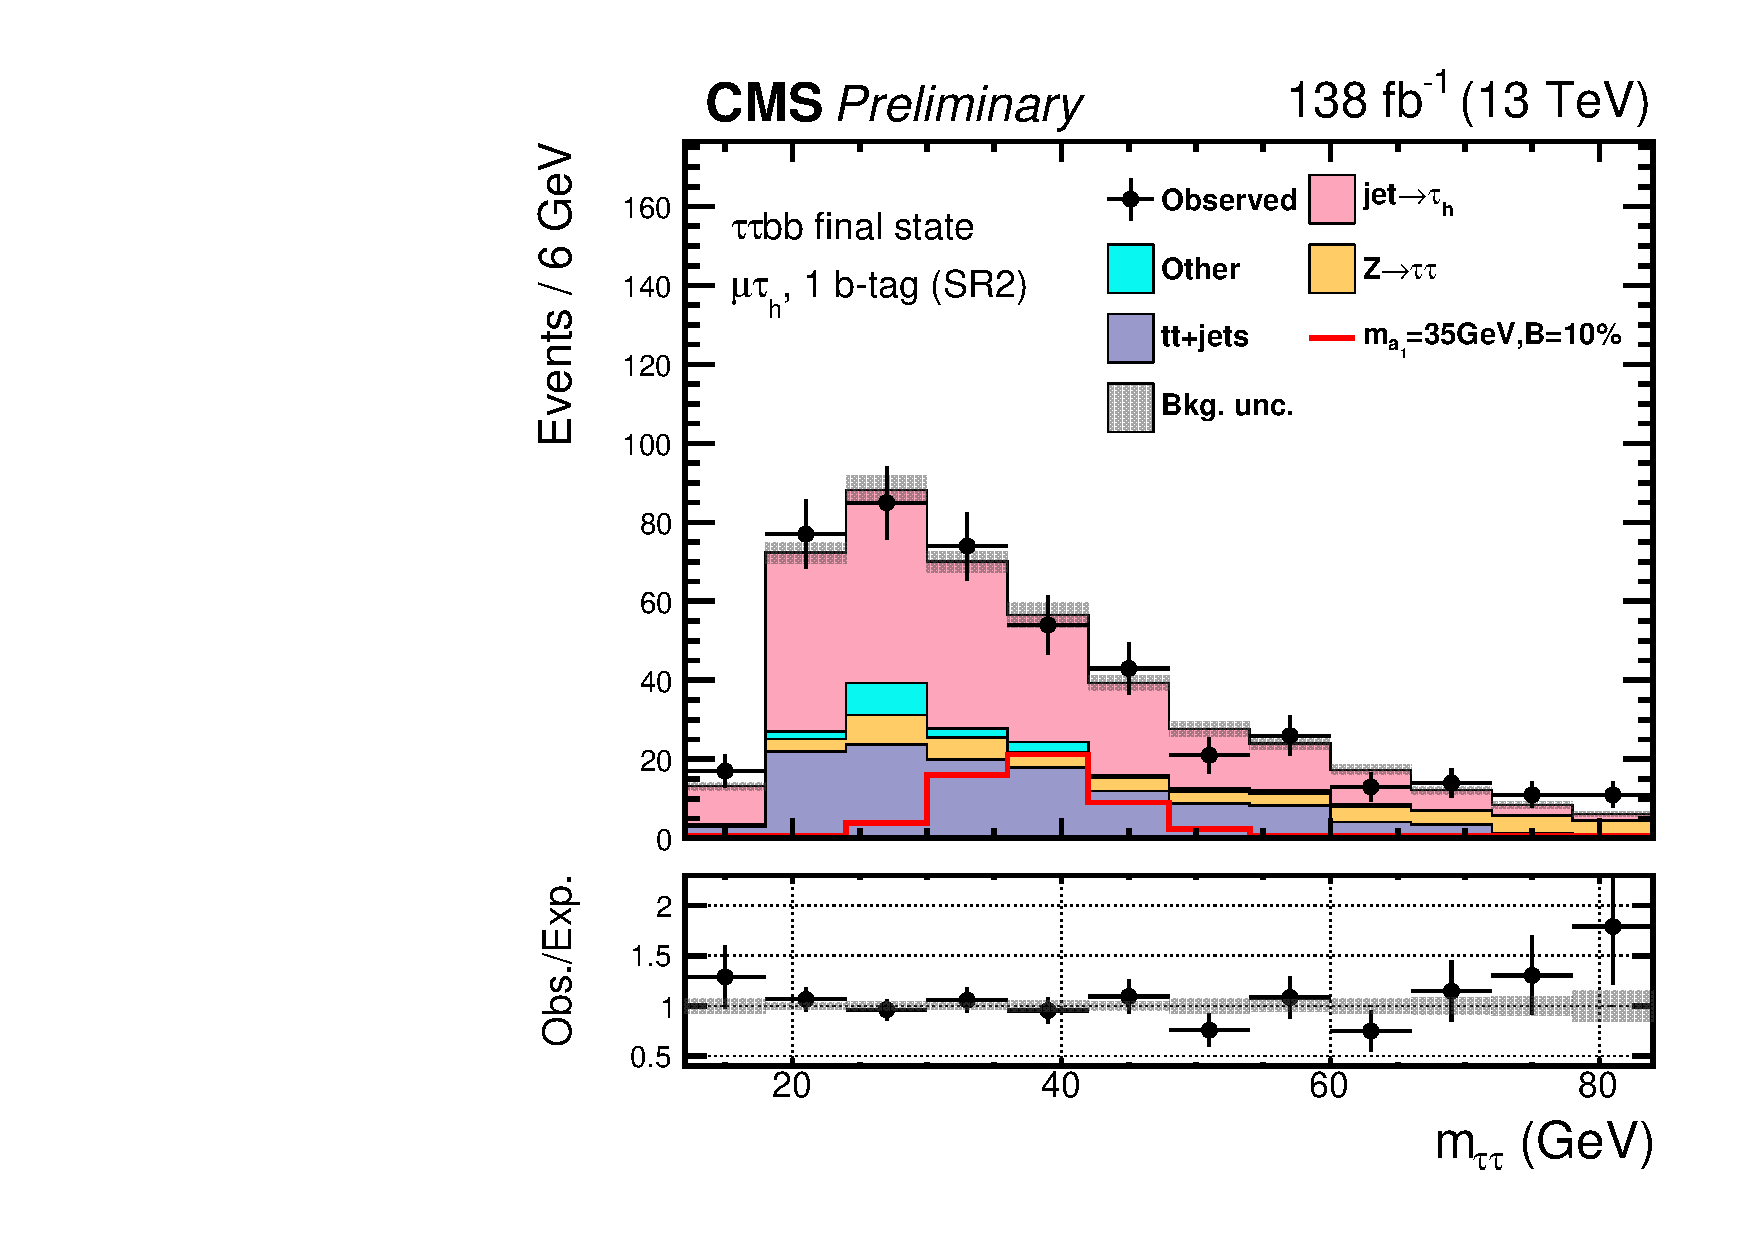
\includegraphics[width=0.32\textwidth]{figures/ch-13-results/mt_all_2_post_prelim-yes.pdf}
        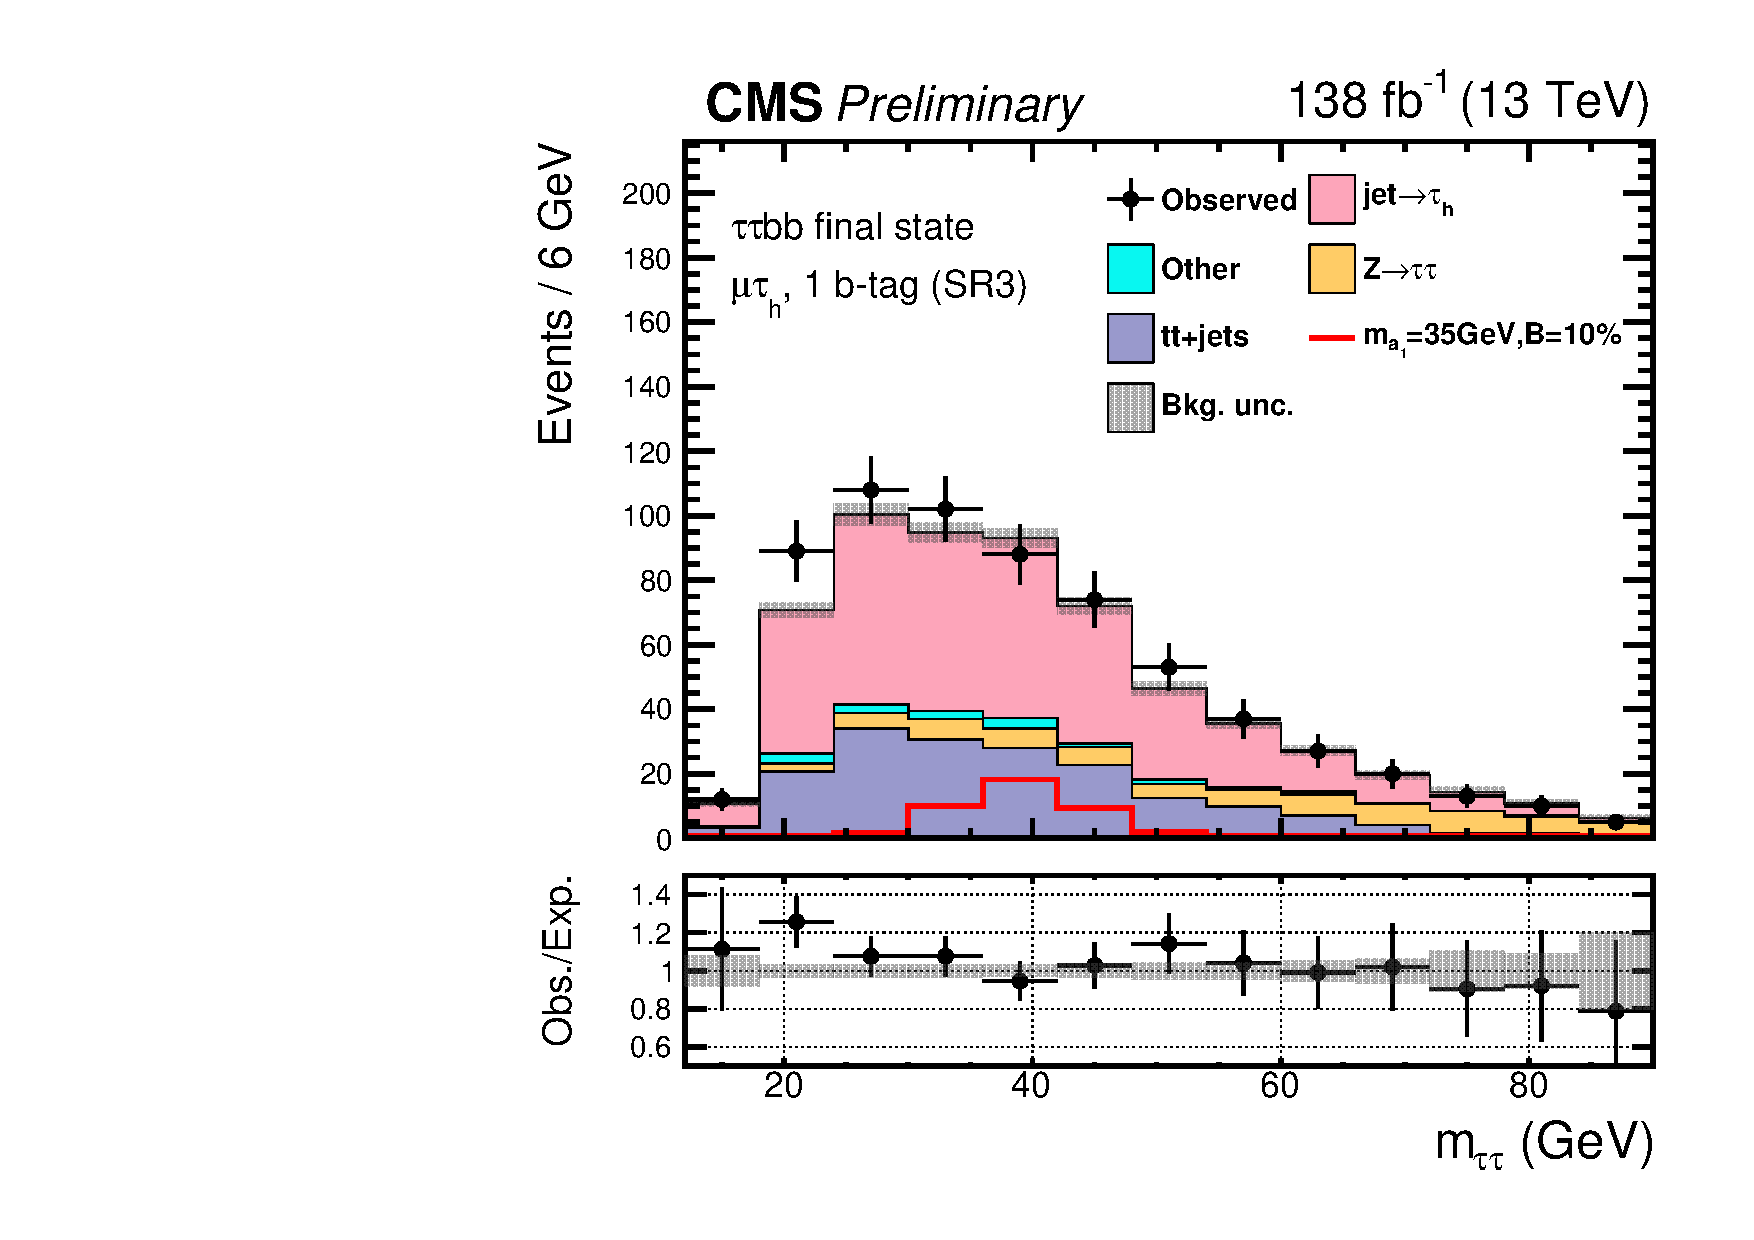
\includegraphics[width=0.32\textwidth]{figures/ch-13-results/mt_all_3_post_prelim-yes.pdf}\\
        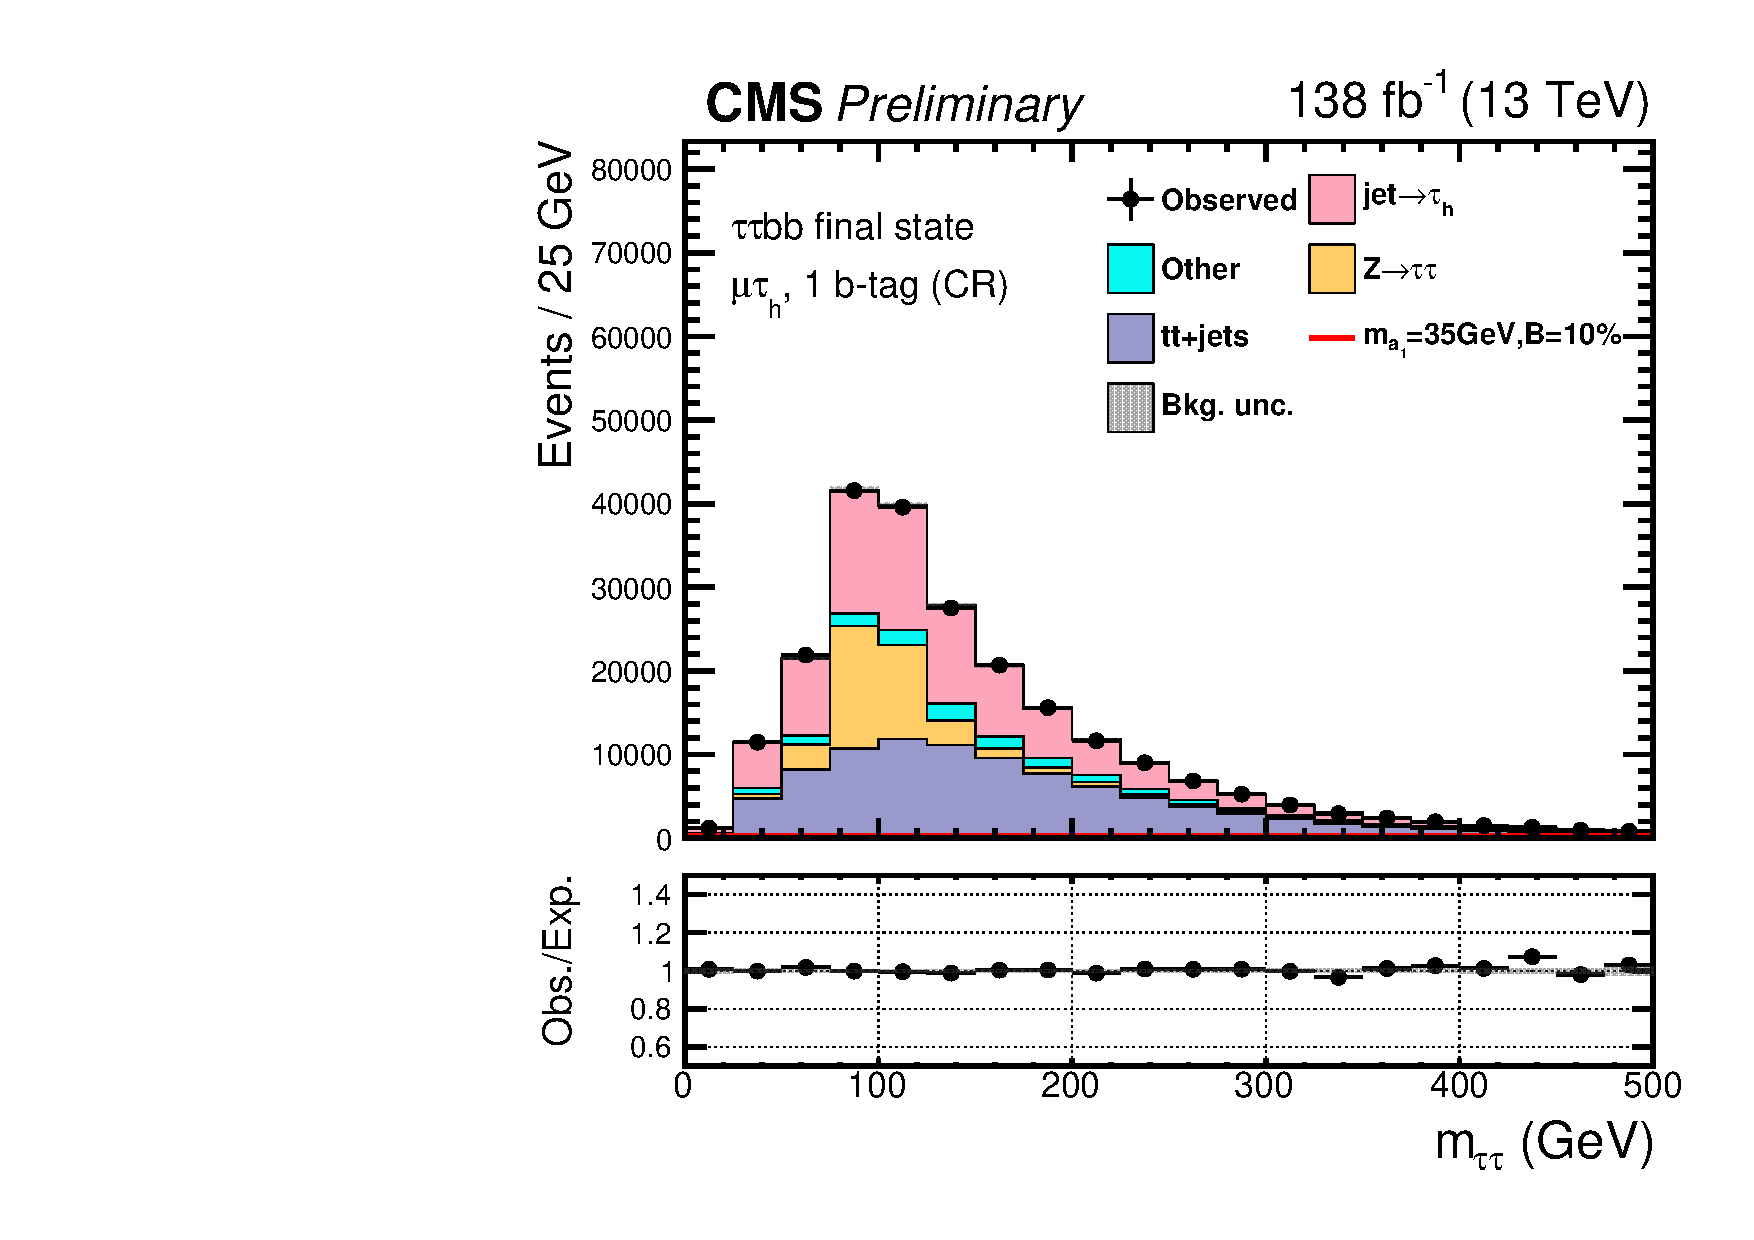
\includegraphics[width=0.32\textwidth]{figures/ch-13-results/mt_all_4_post_prelim-yes.pdf}
        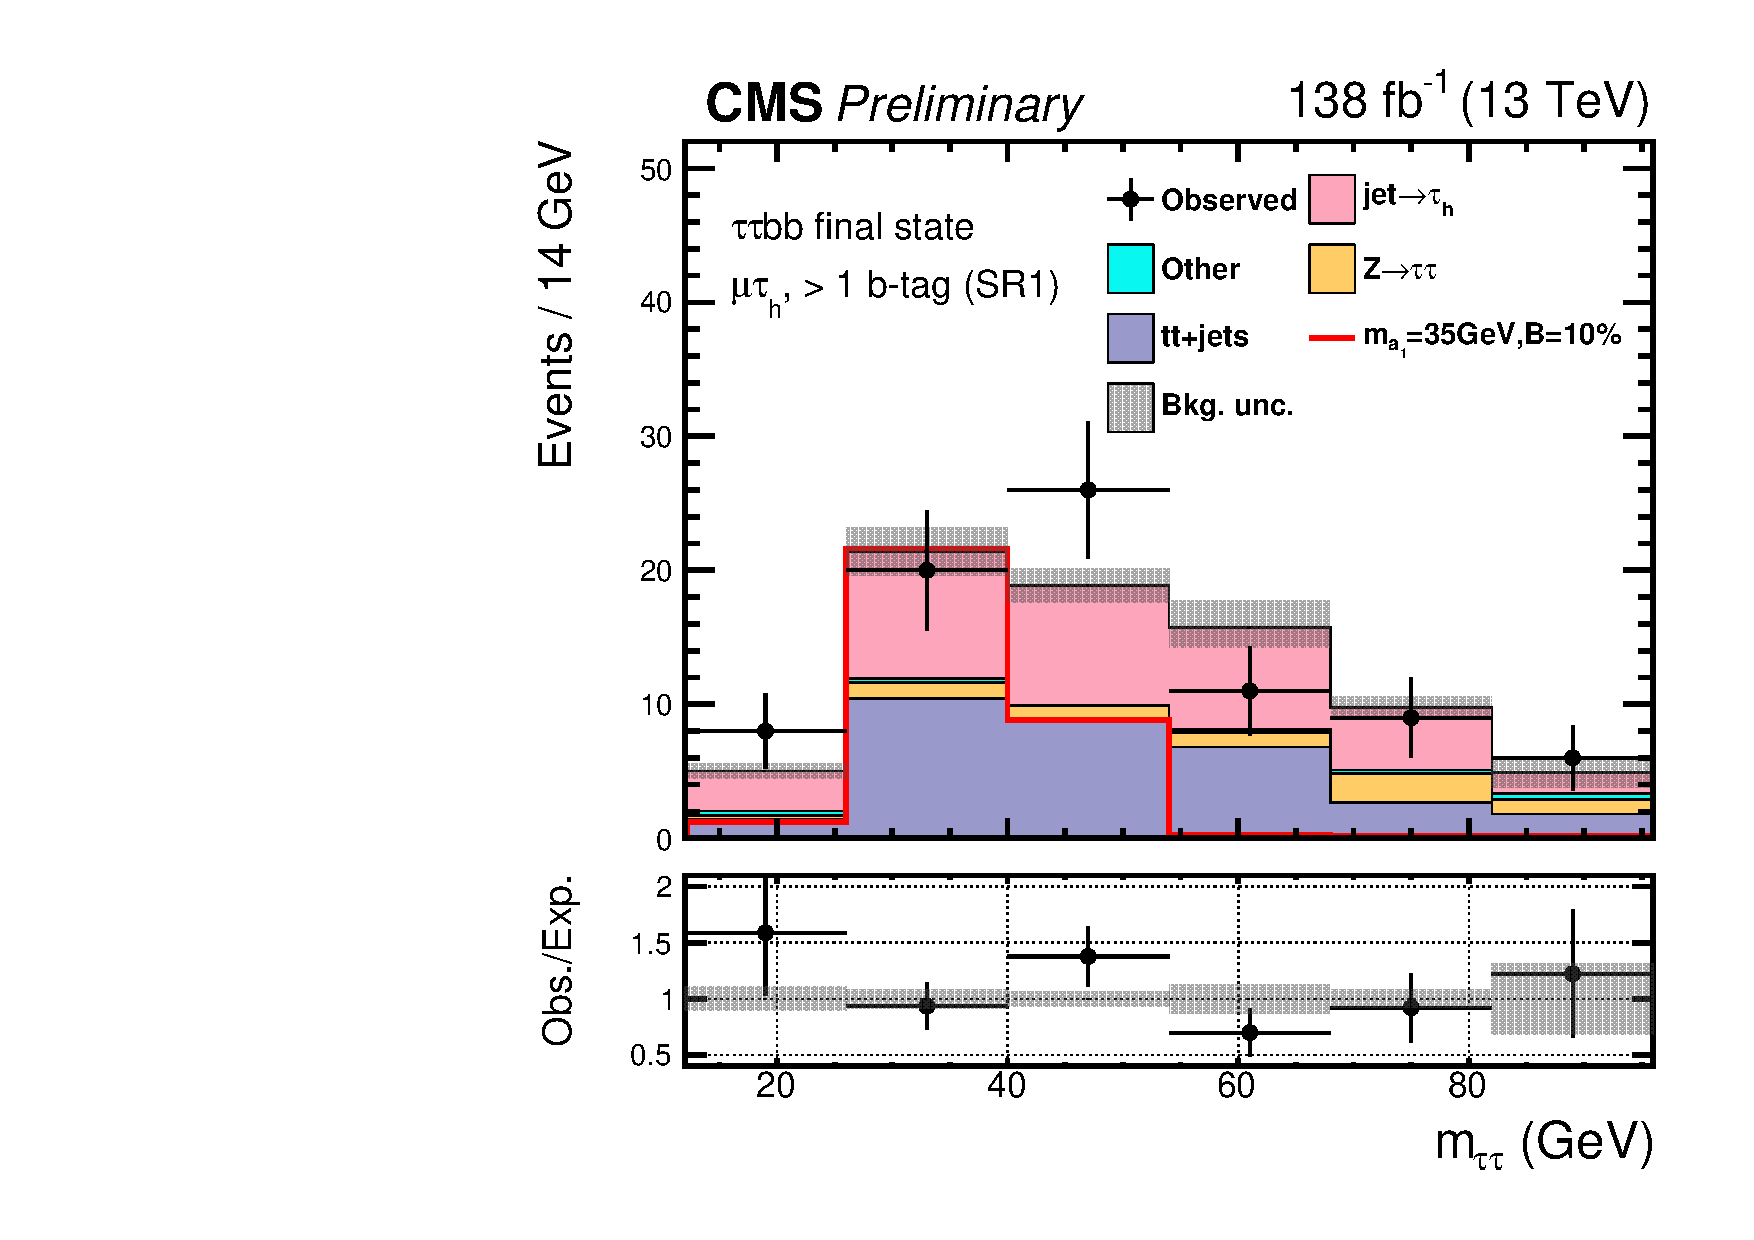
\includegraphics[width=0.32\textwidth]{figures/ch-13-results/mt_all_5_post_prelim-yes.pdf}
        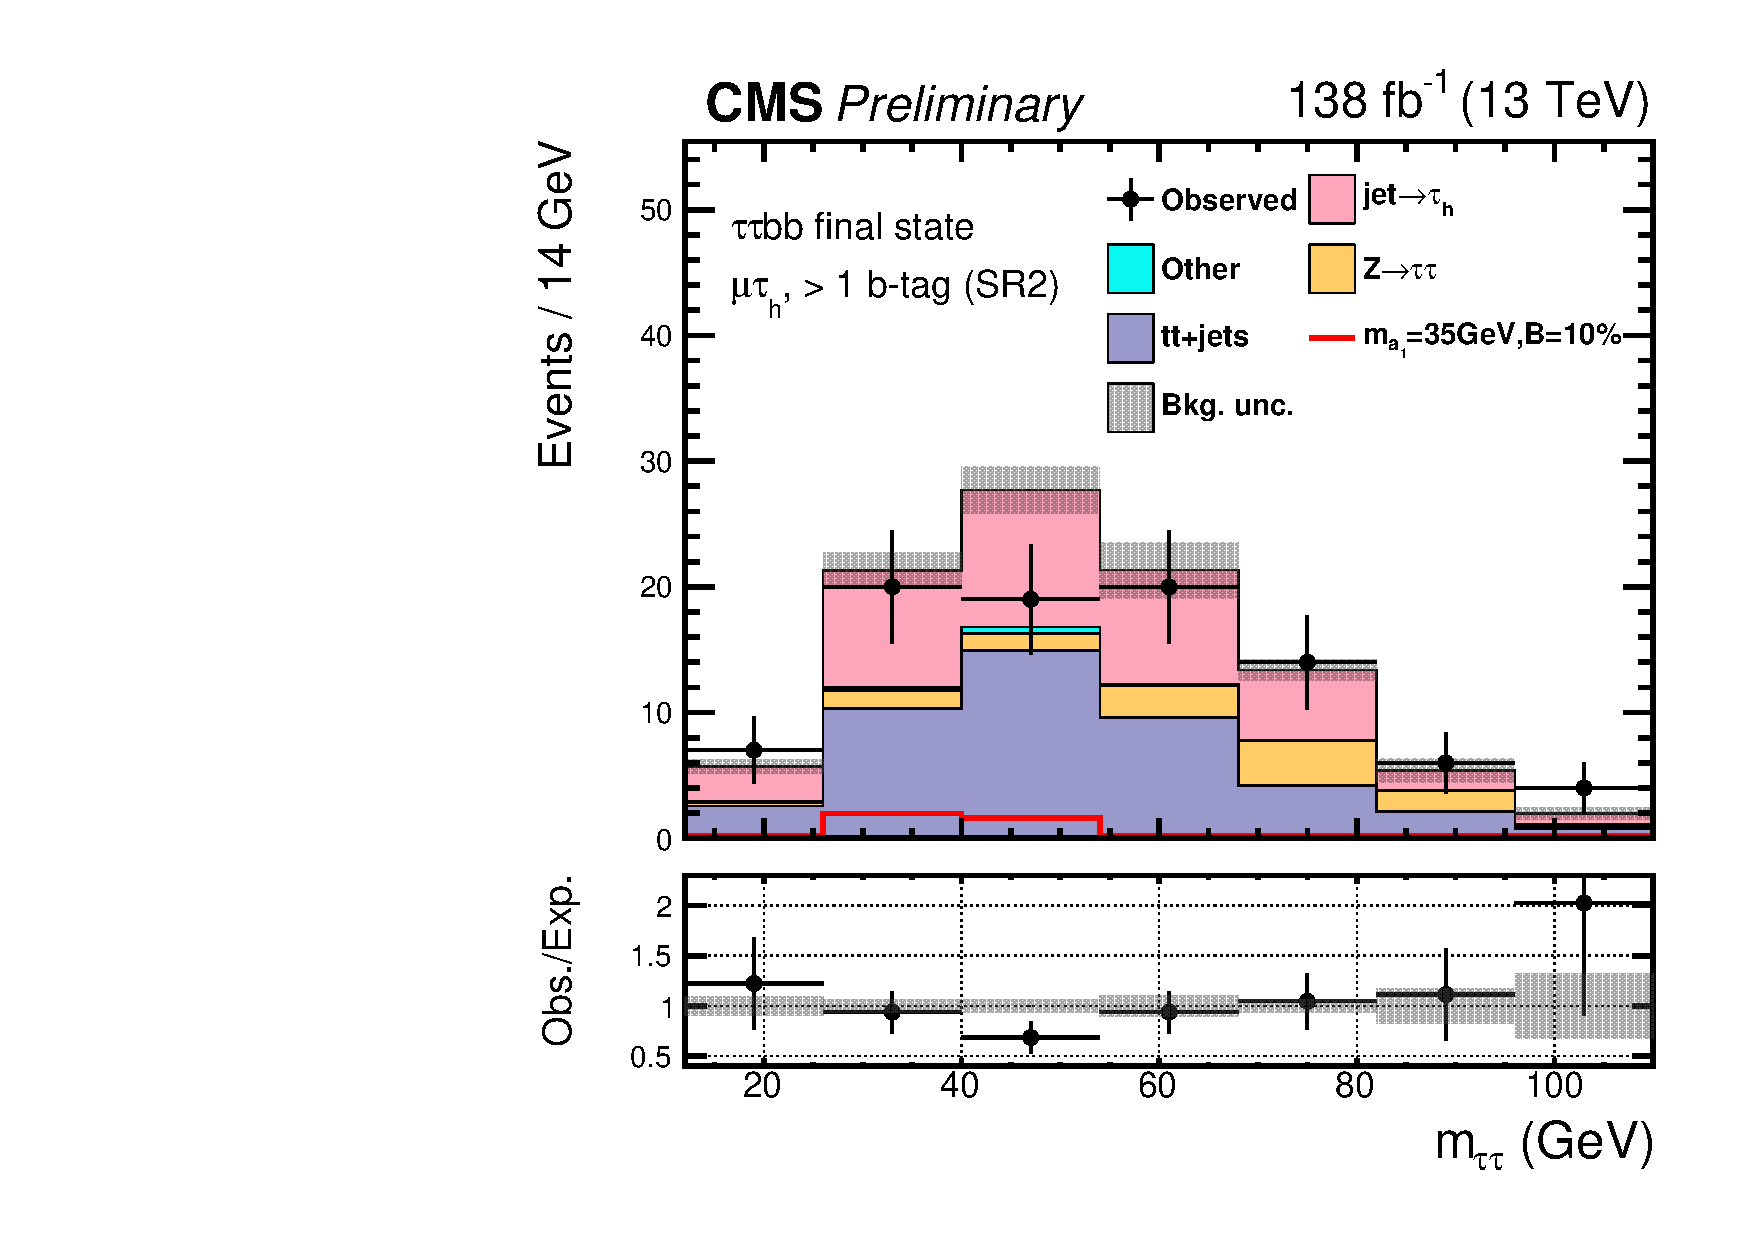
\includegraphics[width=0.32\textwidth]{figures/ch-13-results/mt_all_6_post_prelim-yes.pdf}\\
        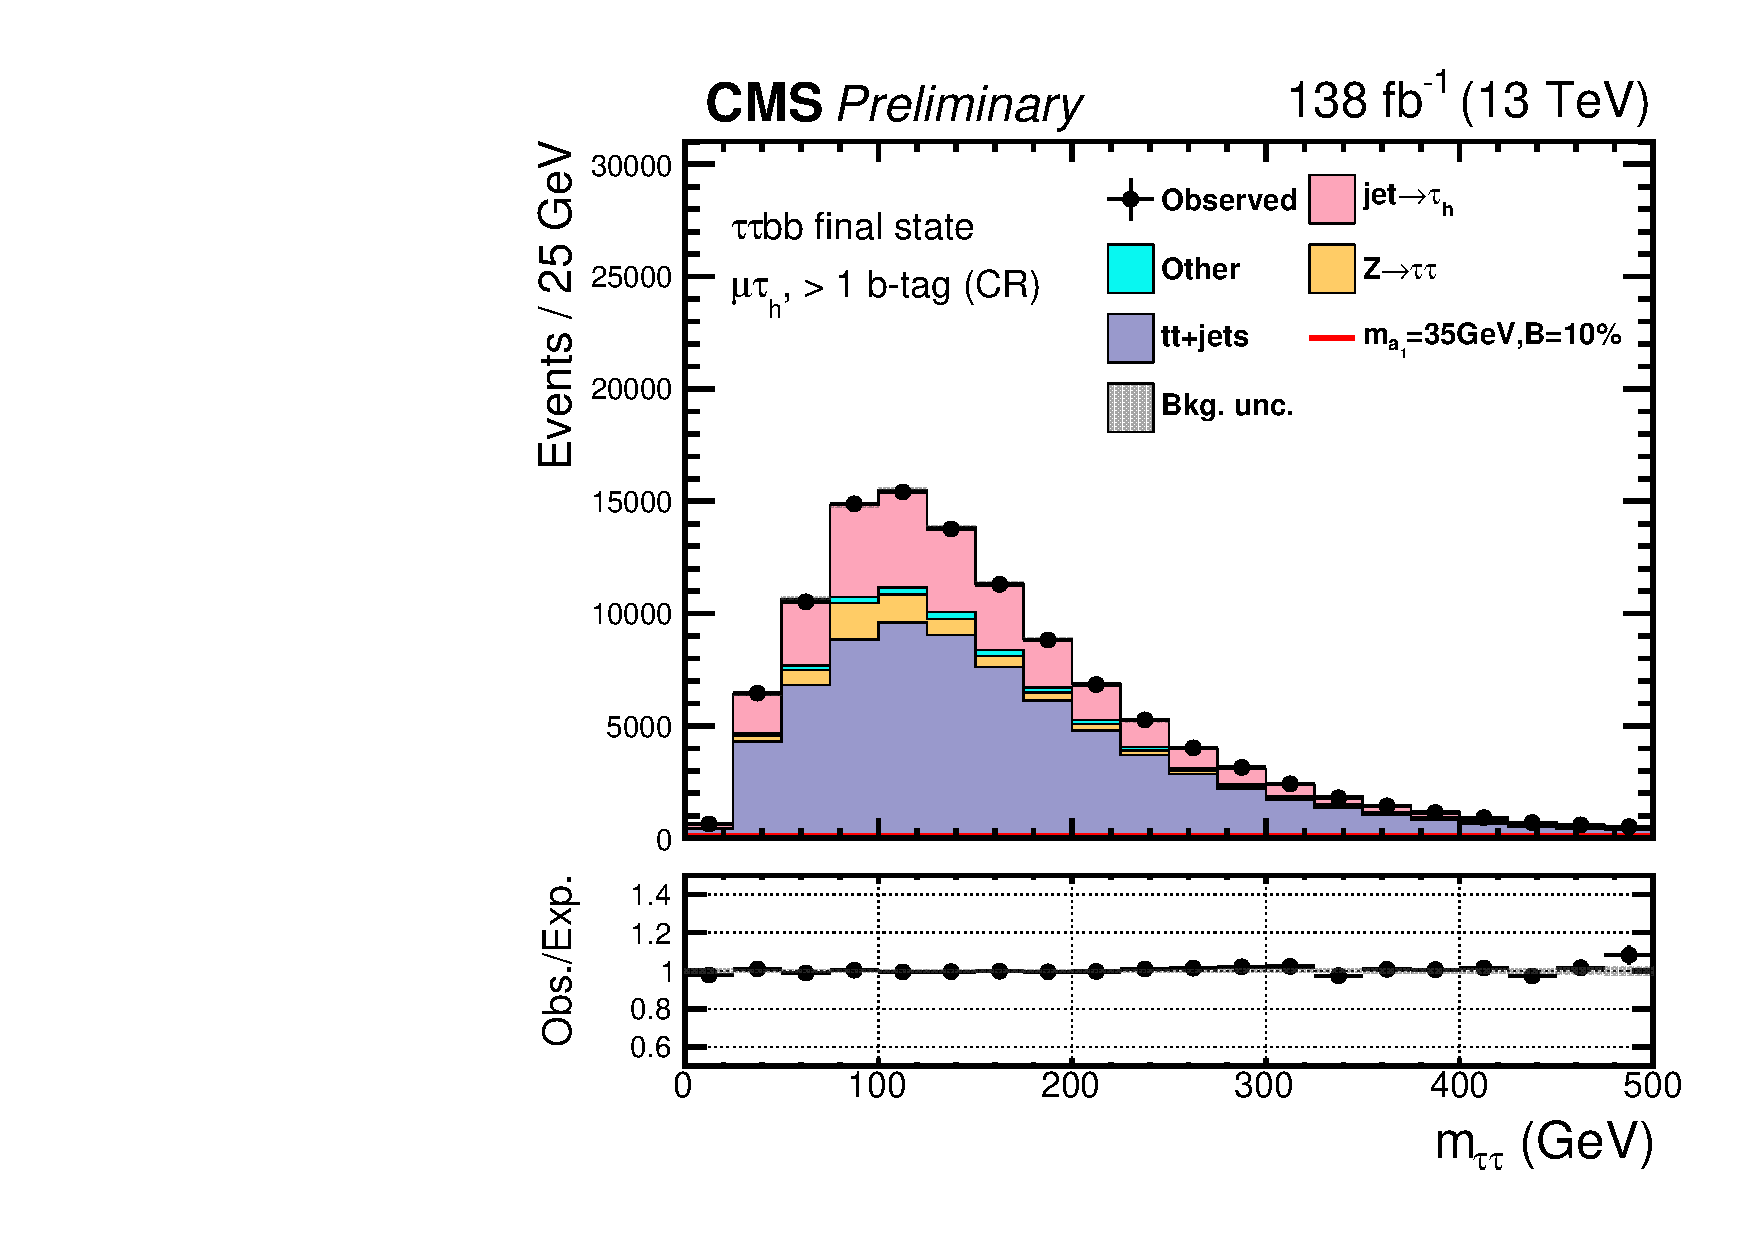
\includegraphics[width=0.32\textwidth]{figures/ch-13-results/mt_all_7_post_prelim-yes.pdf}
    \end{center}
    \caption[Postfit final $m_{\tau\tau}$ distributions in the $\mu\tau_{h}$ channel.]{Postfit final $m_{\tau\tau}$ distributions in the $\mu\tau_{h}$ channel \cite{CMS-AN-20-213}. Statistical and systematic uncertainties are included. \textit{Top row:} 1 b-tag jet categories: three signal regions (SR1, SR2, SR3). \textit{Middle row, left to right:} 1 b-tag jet categories: control region (CR), and 2 b-tag jet categories: two signal regions (SR1, SR2). \textit{Bottom:} 2 b-tag jet categories: control region (CR).}
    \label{fig:results_mtt_postfit_mtall}
\end{figure}

\begin{figure}[ht]
    \begin{center}
        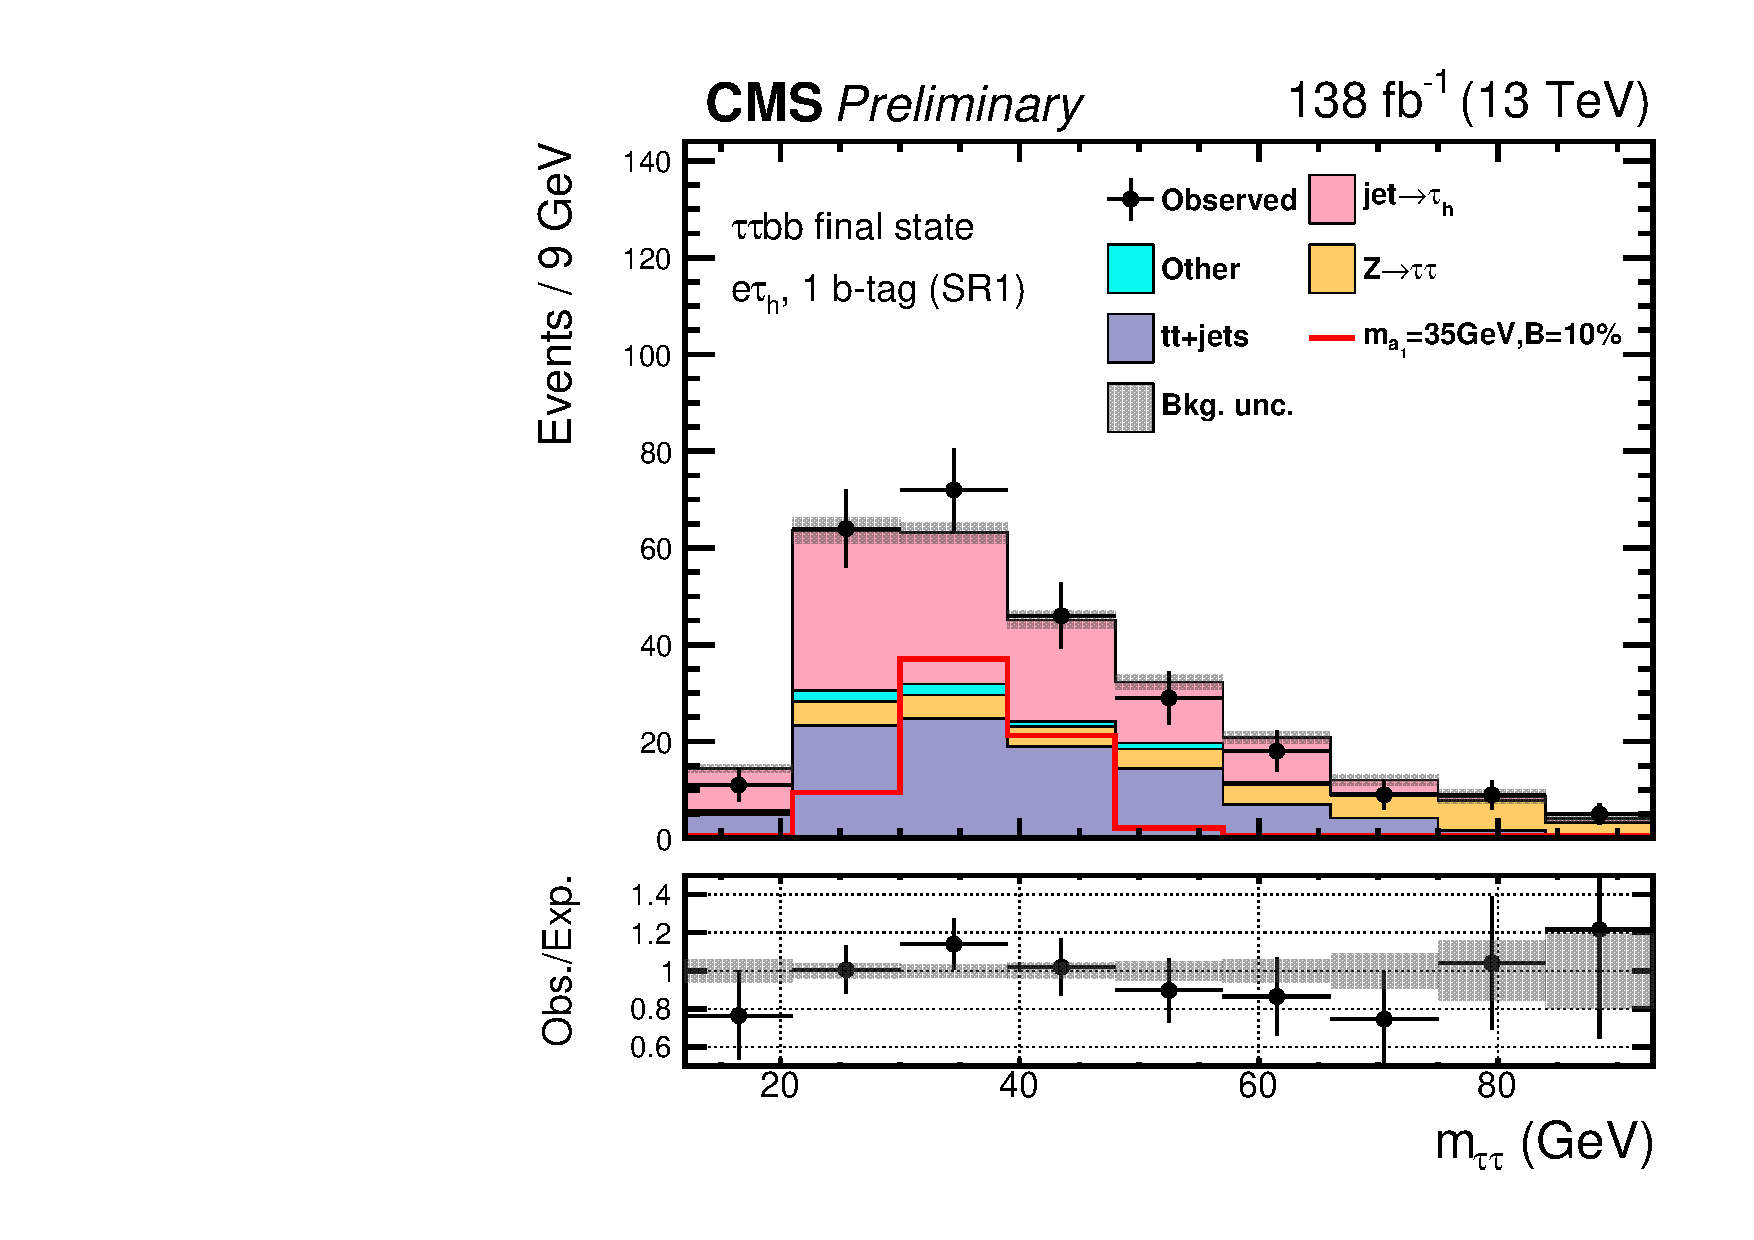
\includegraphics[width=0.32\textwidth]{figures/ch-13-results/et_all_1_post_prelim-yes.pdf}
        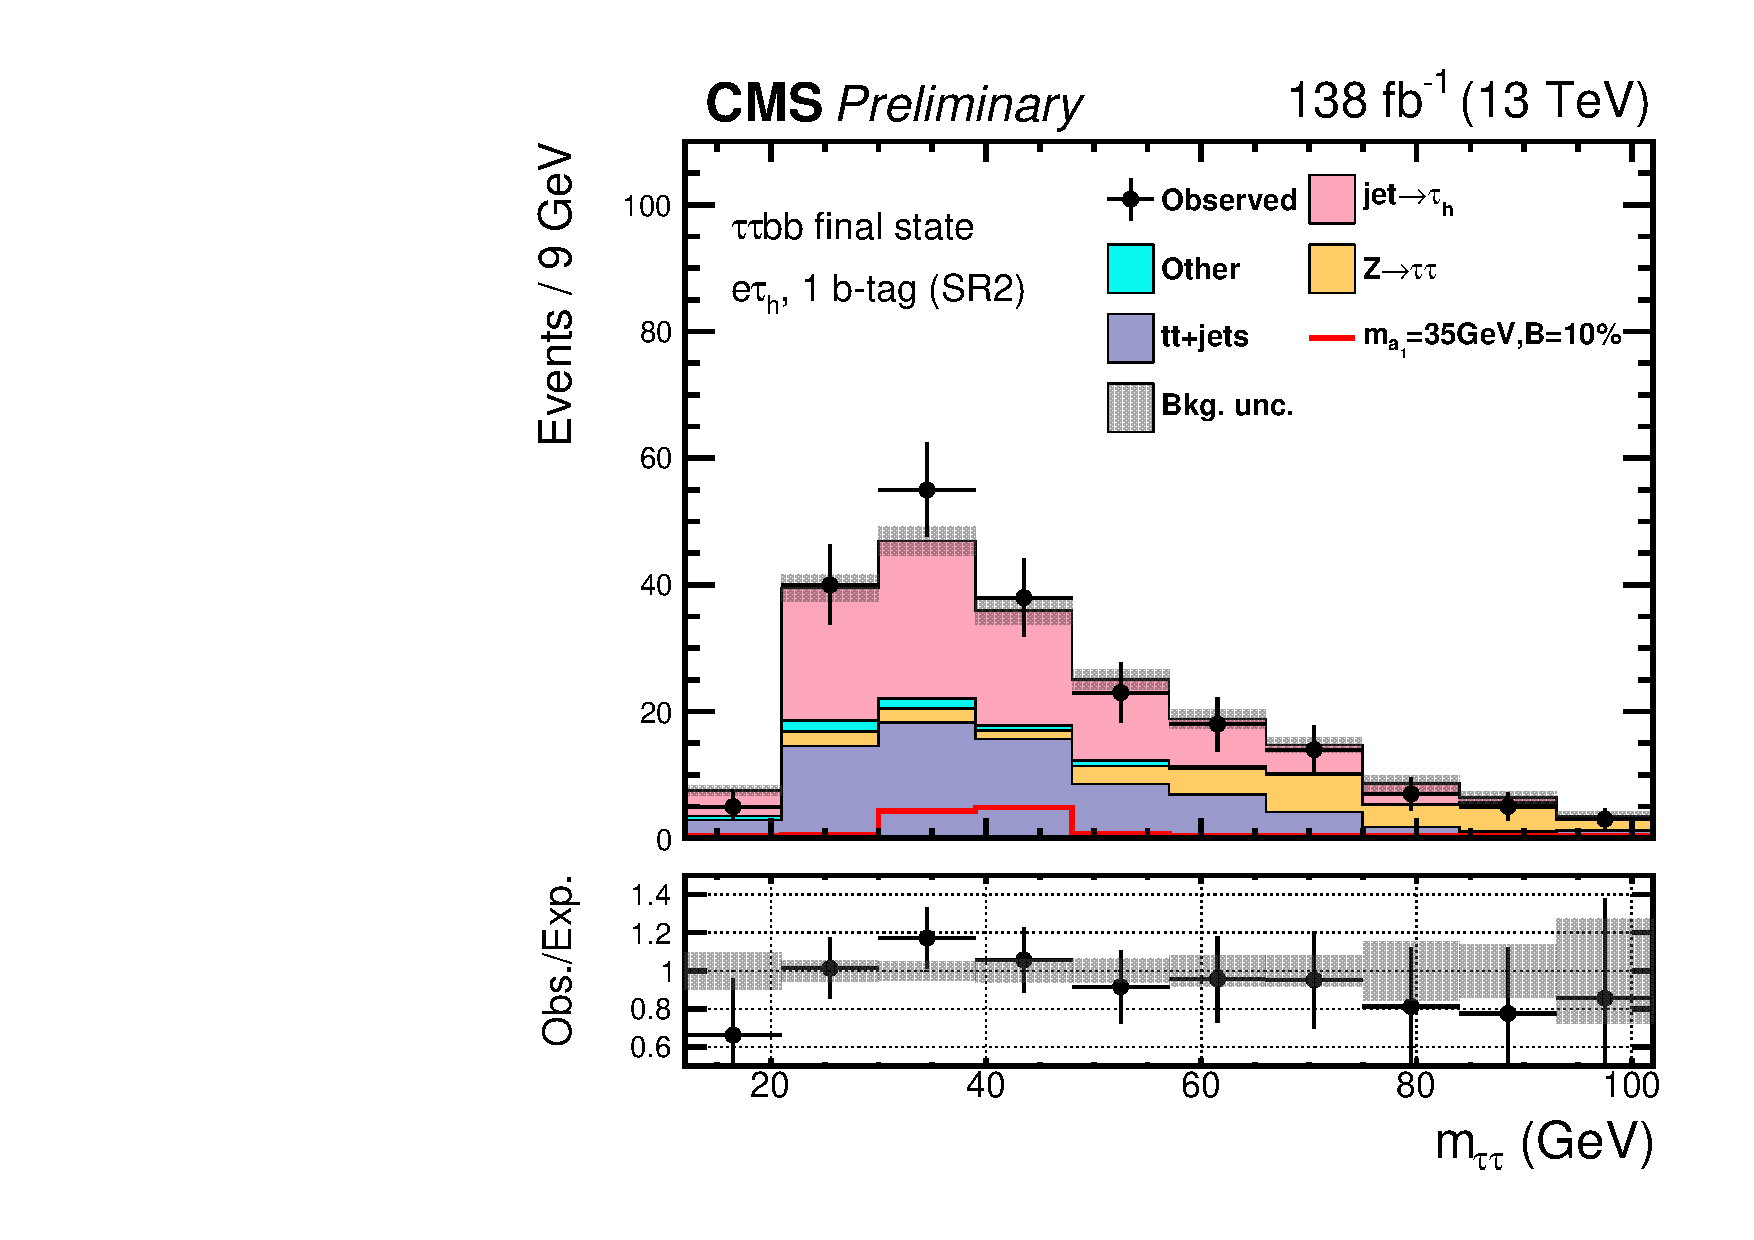
\includegraphics[width=0.32\textwidth]{figures/ch-13-results/et_all_2_post_prelim-yes.pdf}
        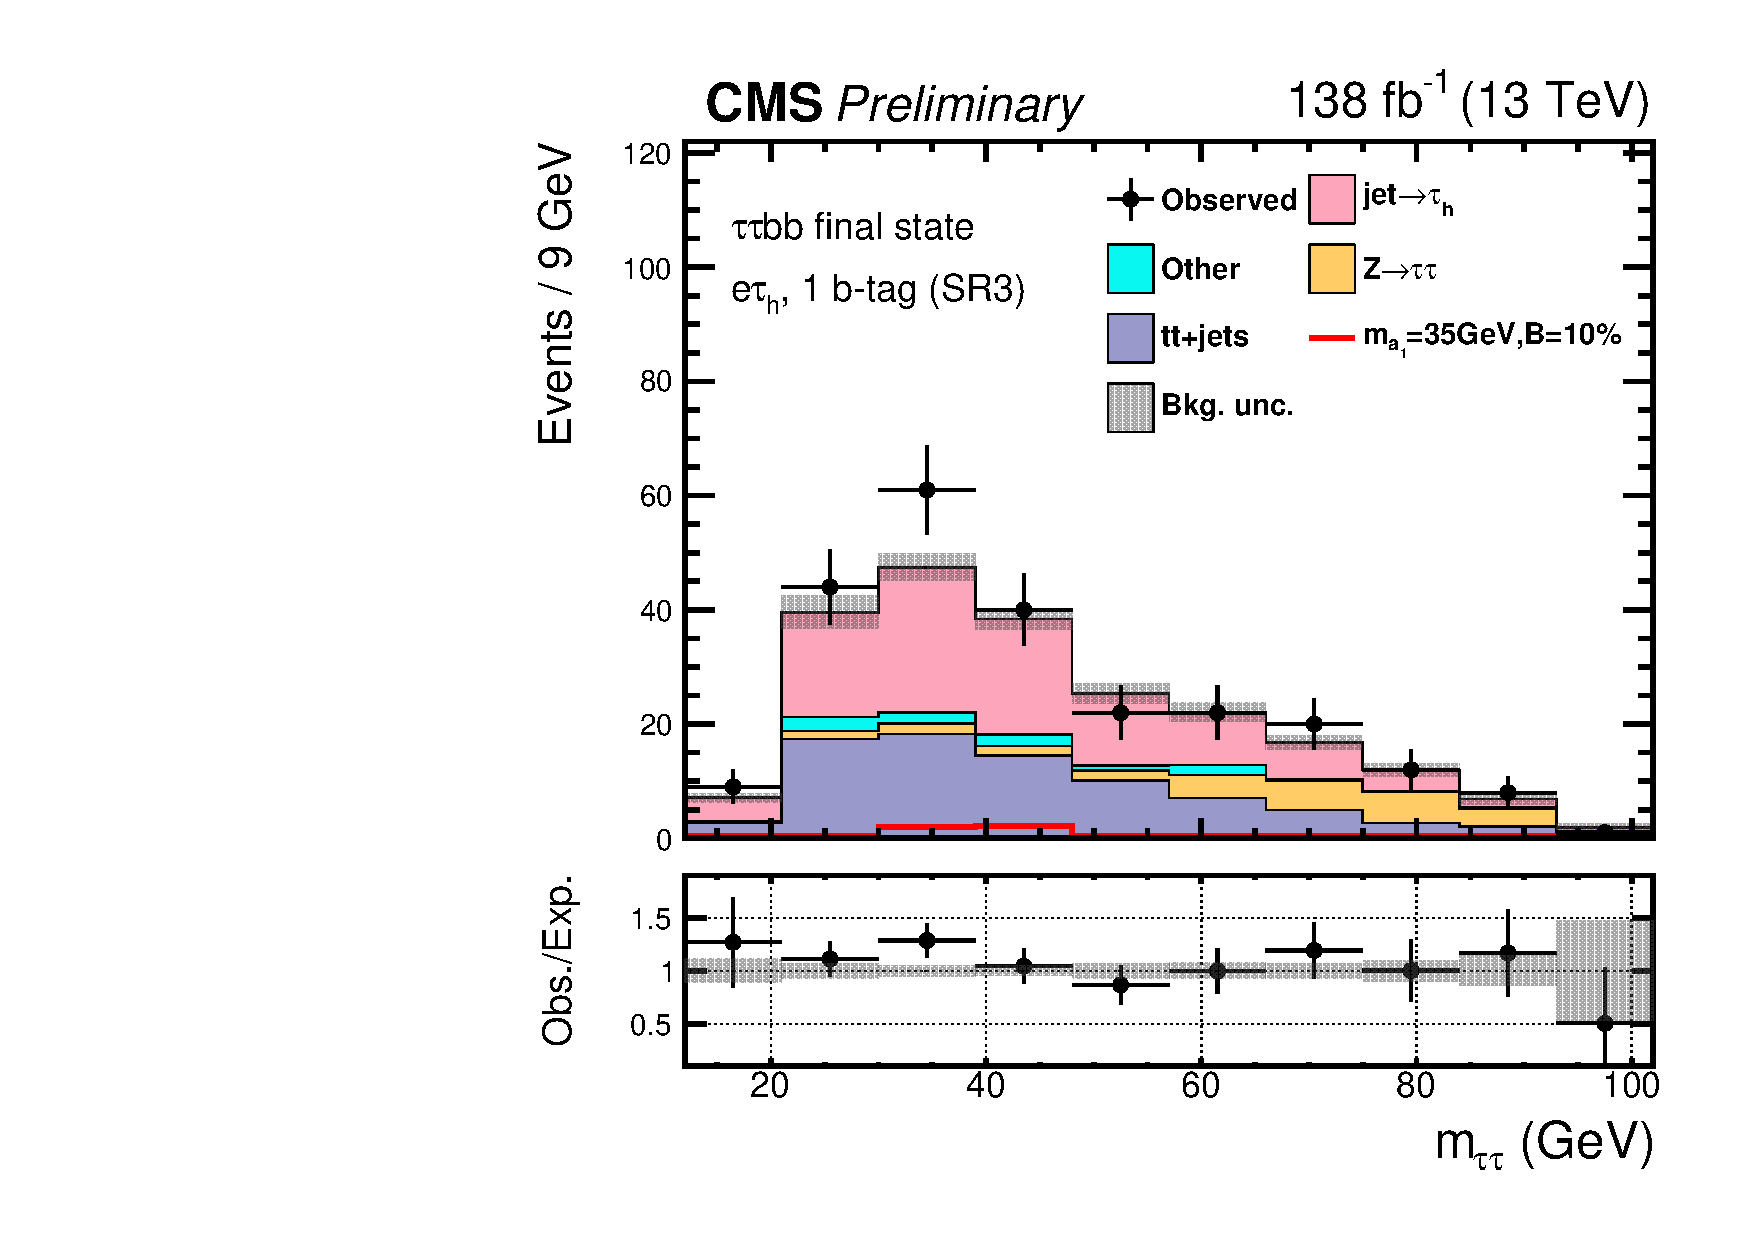
\includegraphics[width=0.32\textwidth]{figures/ch-13-results/et_all_3_post_prelim-yes.pdf}\\
        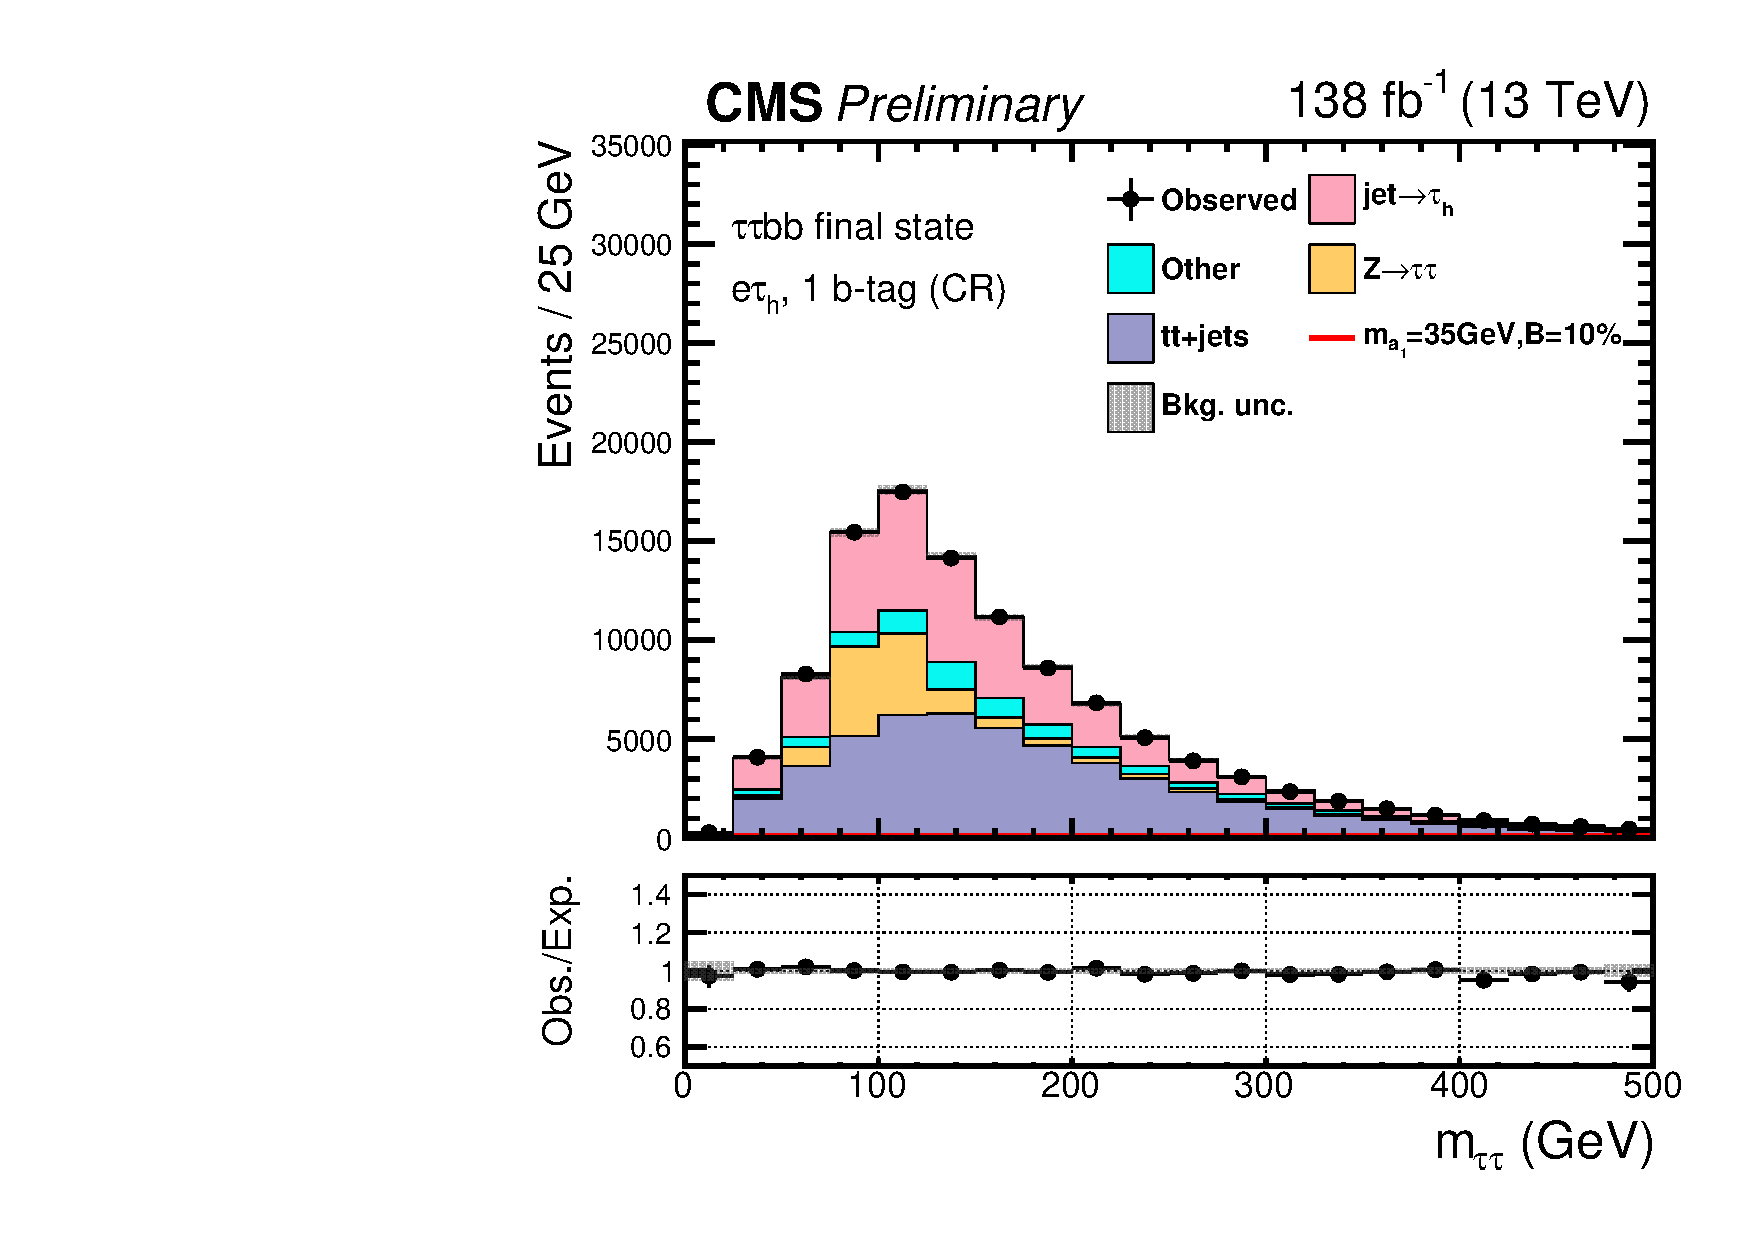
\includegraphics[width=0.32\textwidth]{figures/ch-13-results/et_all_4_post_prelim-yes.pdf}
        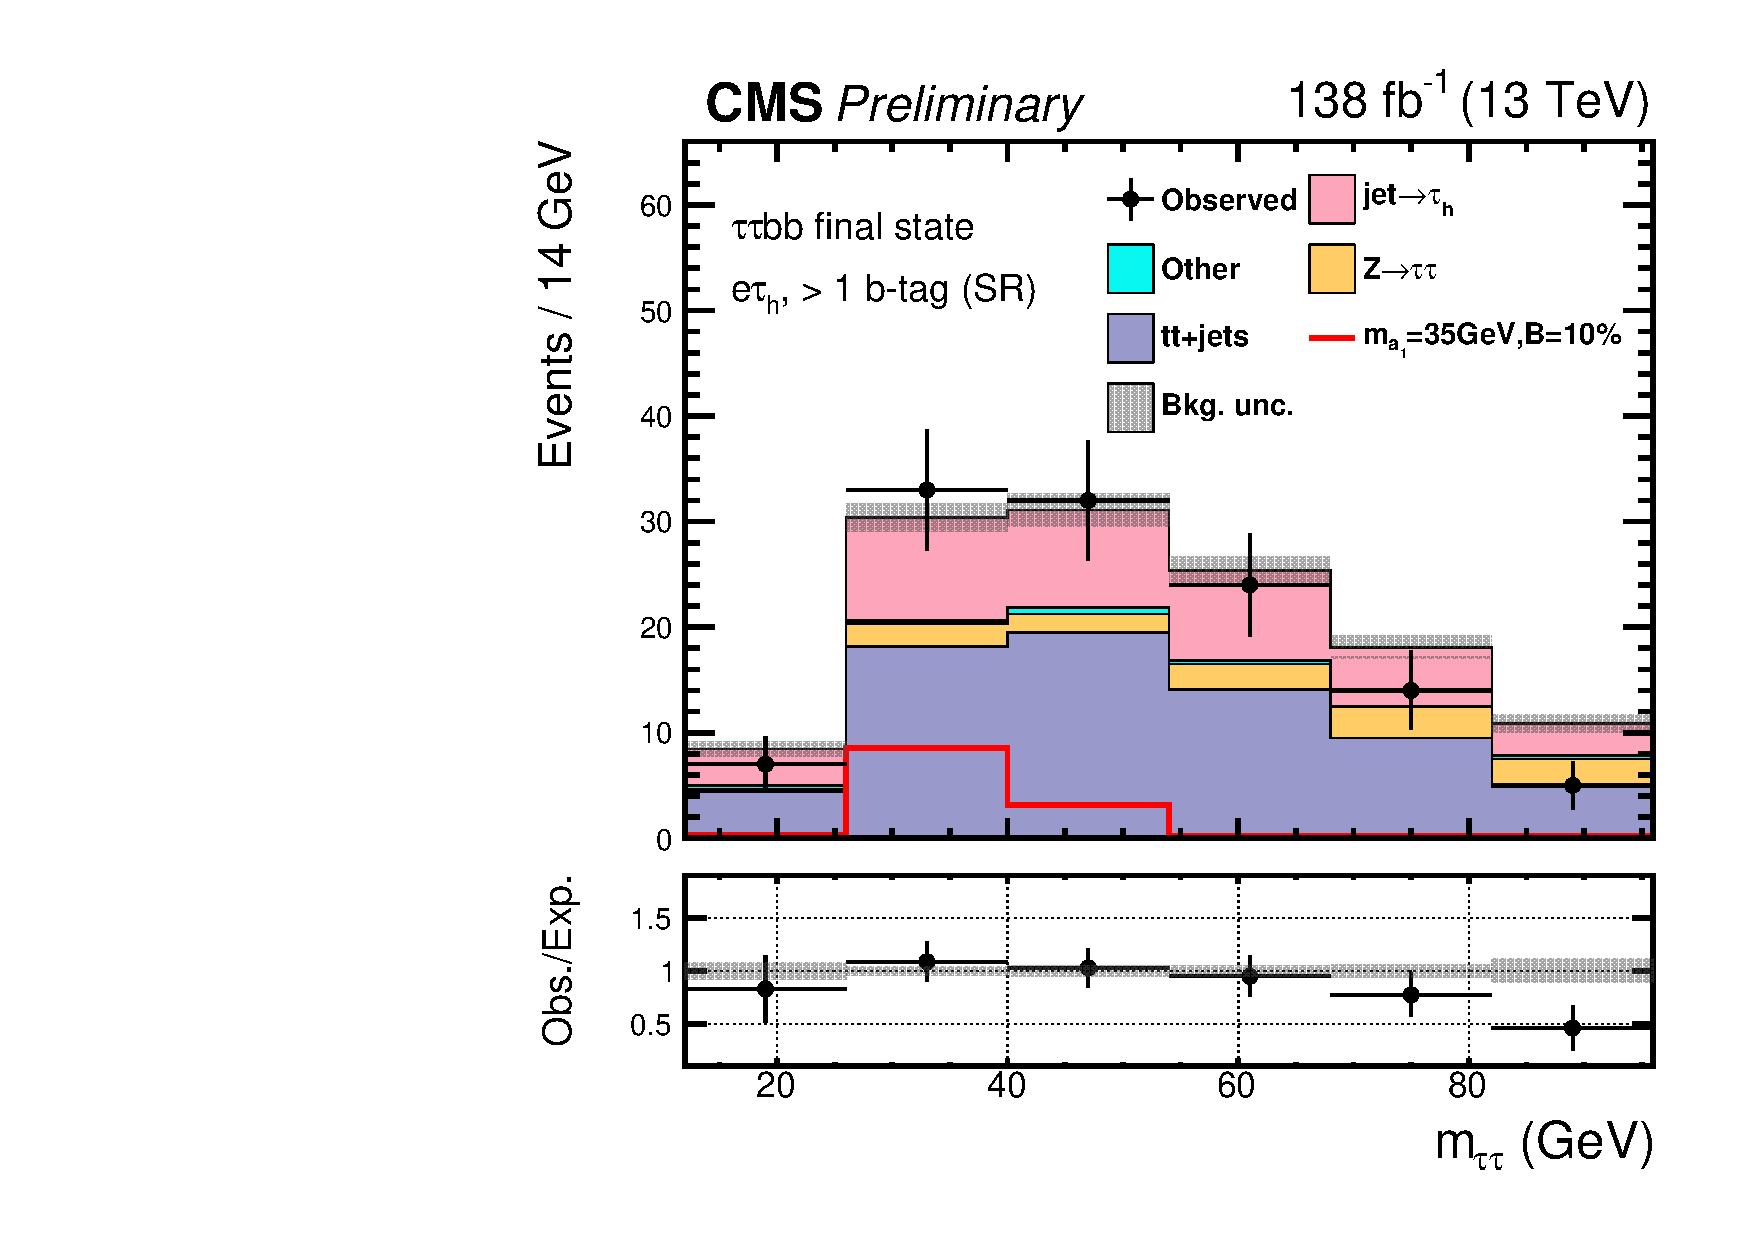
\includegraphics[width=0.32\textwidth]{figures/ch-13-results/et_all_5_post_prelim-yes.pdf}
        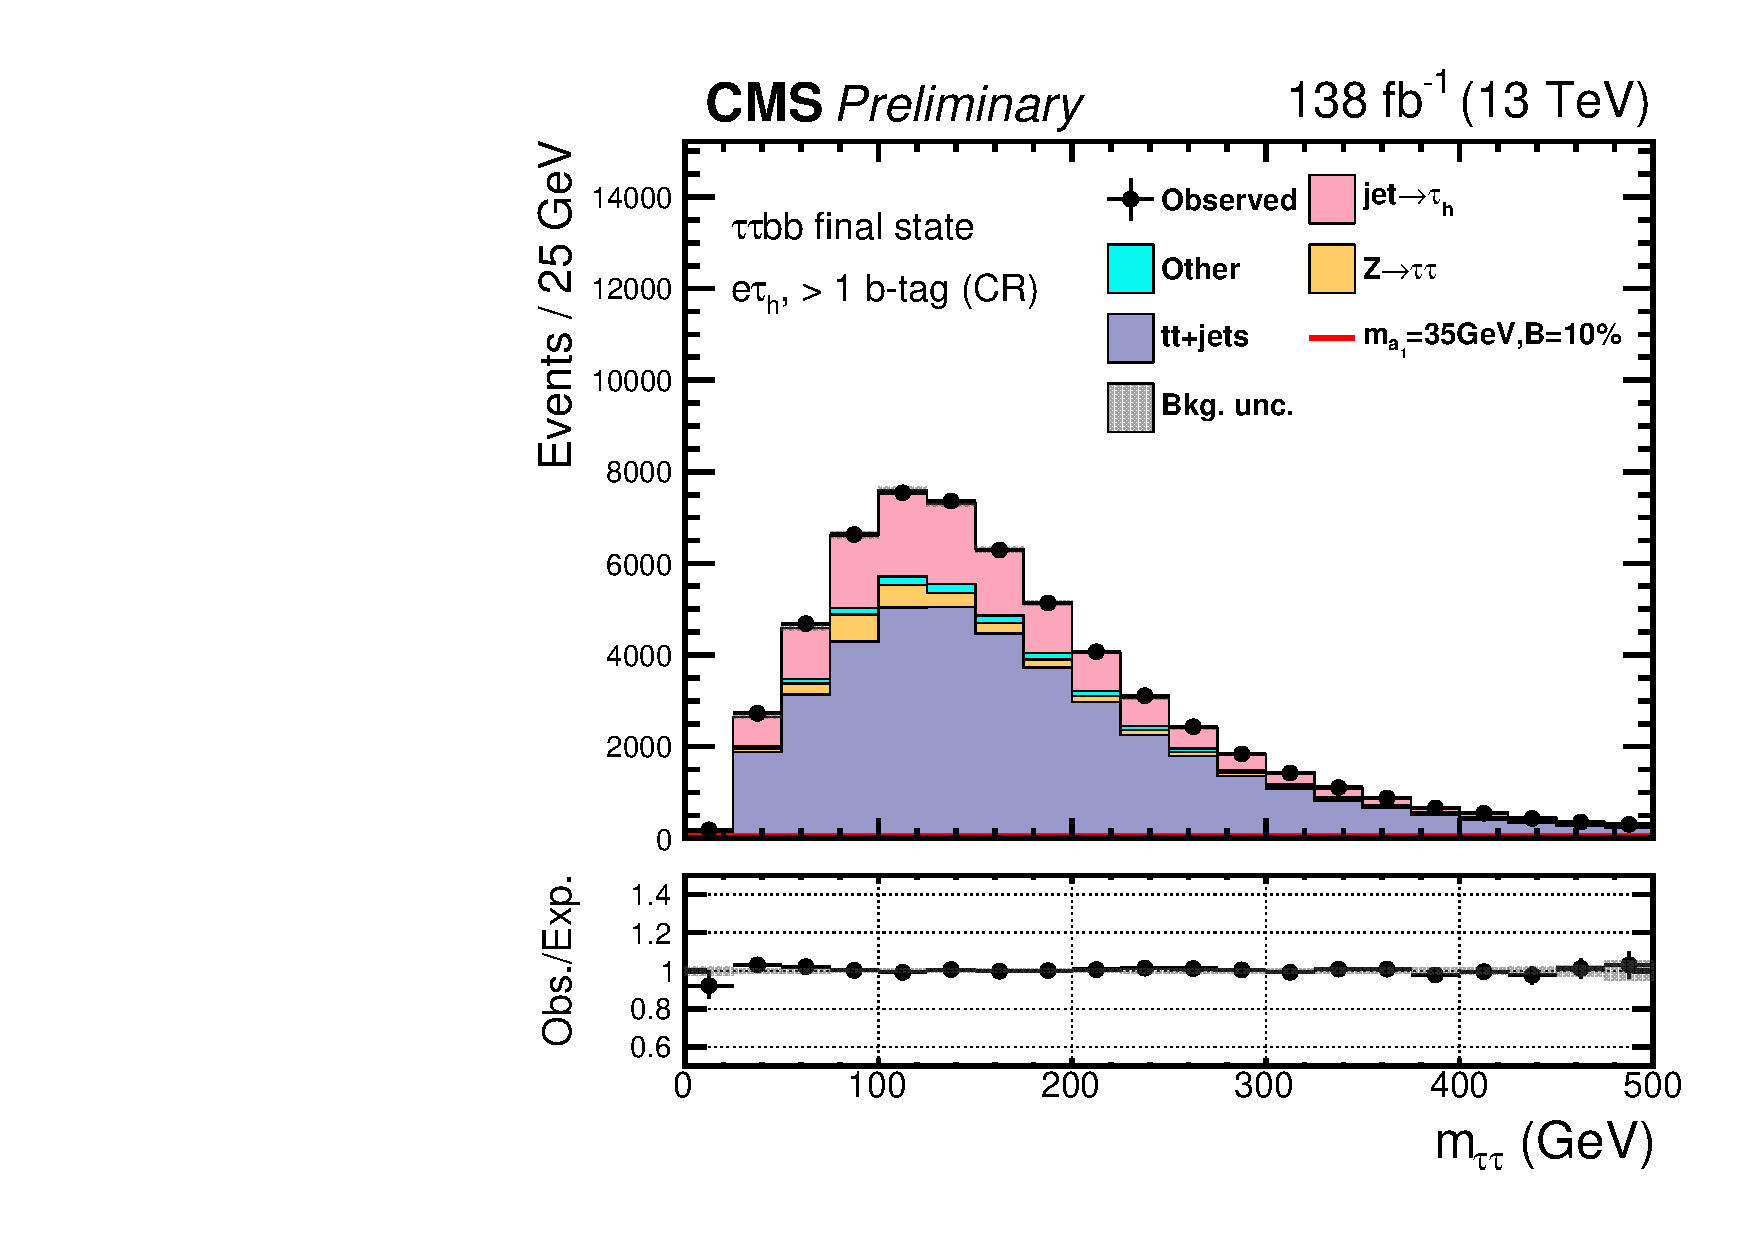
\includegraphics[width=0.32\textwidth]{figures/ch-13-results/et_all_6_post_prelim-yes.pdf}
    \end{center}
    \caption[Postfit final $m_{\tau\tau}$ distributions in the $e\tau_{h}$ channel]{Postfit final $m_{\tau\tau}$ distributions in the $e\tau_{h}$ channel \cite{CMS-AN-20-213}. Statistical and systematic uncertainties are included. \textit{Top row:} 1 b-tag jet categories: three signal regions (SR1, SR2, SR3). \textit{Bottom row, left to right:} 1-btag jet categories: control region (CR), and 2 b-tag jet categories: signal region (SR) and control region (CR).}
    \label{fig:results_mtt_postfit_etall}
\end{figure}

\begin{figure}[ht]
    \begin{center}
        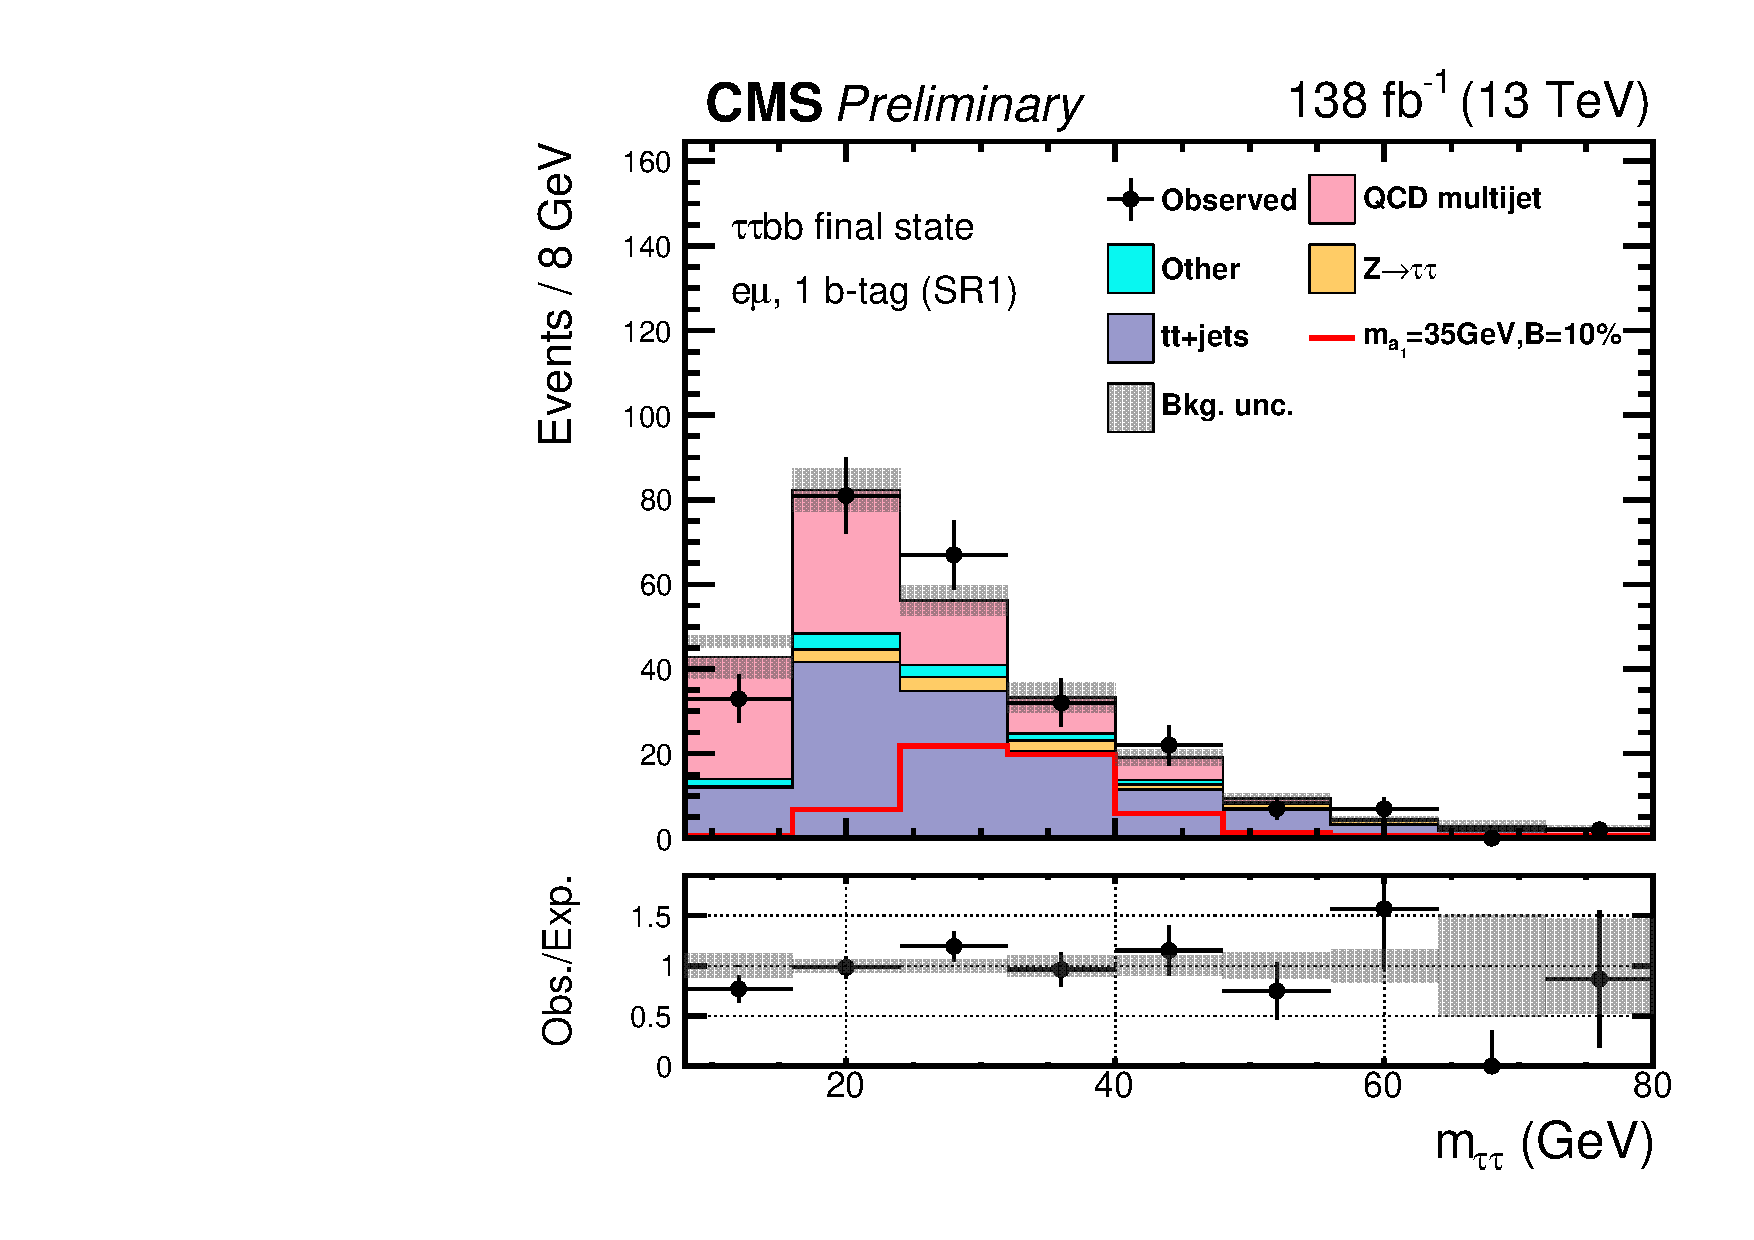
\includegraphics[width=0.32\textwidth]{figures/ch-13-results/em_all_1_post_prelim-yes.pdf}
        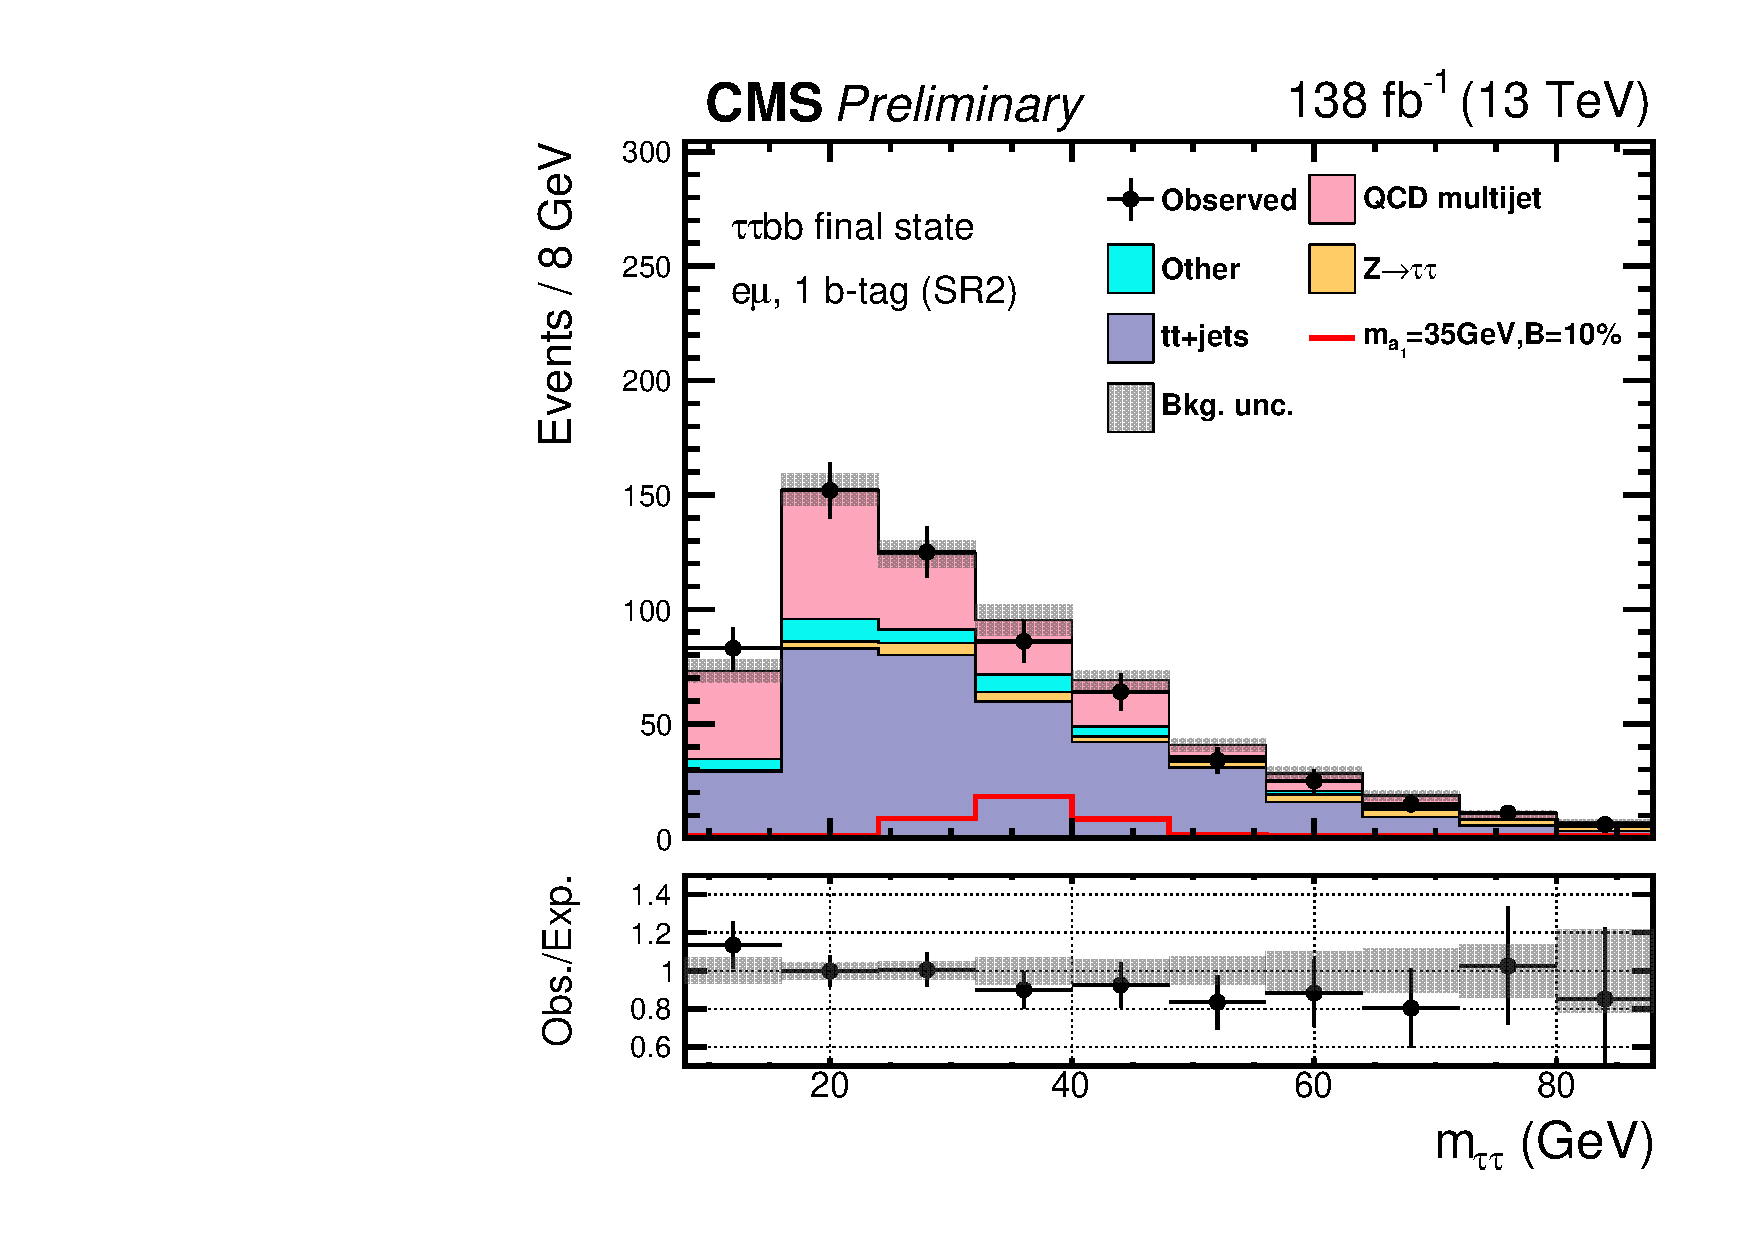
\includegraphics[width=0.32\textwidth]{figures/ch-13-results/em_all_2_post_prelim-yes.pdf}
        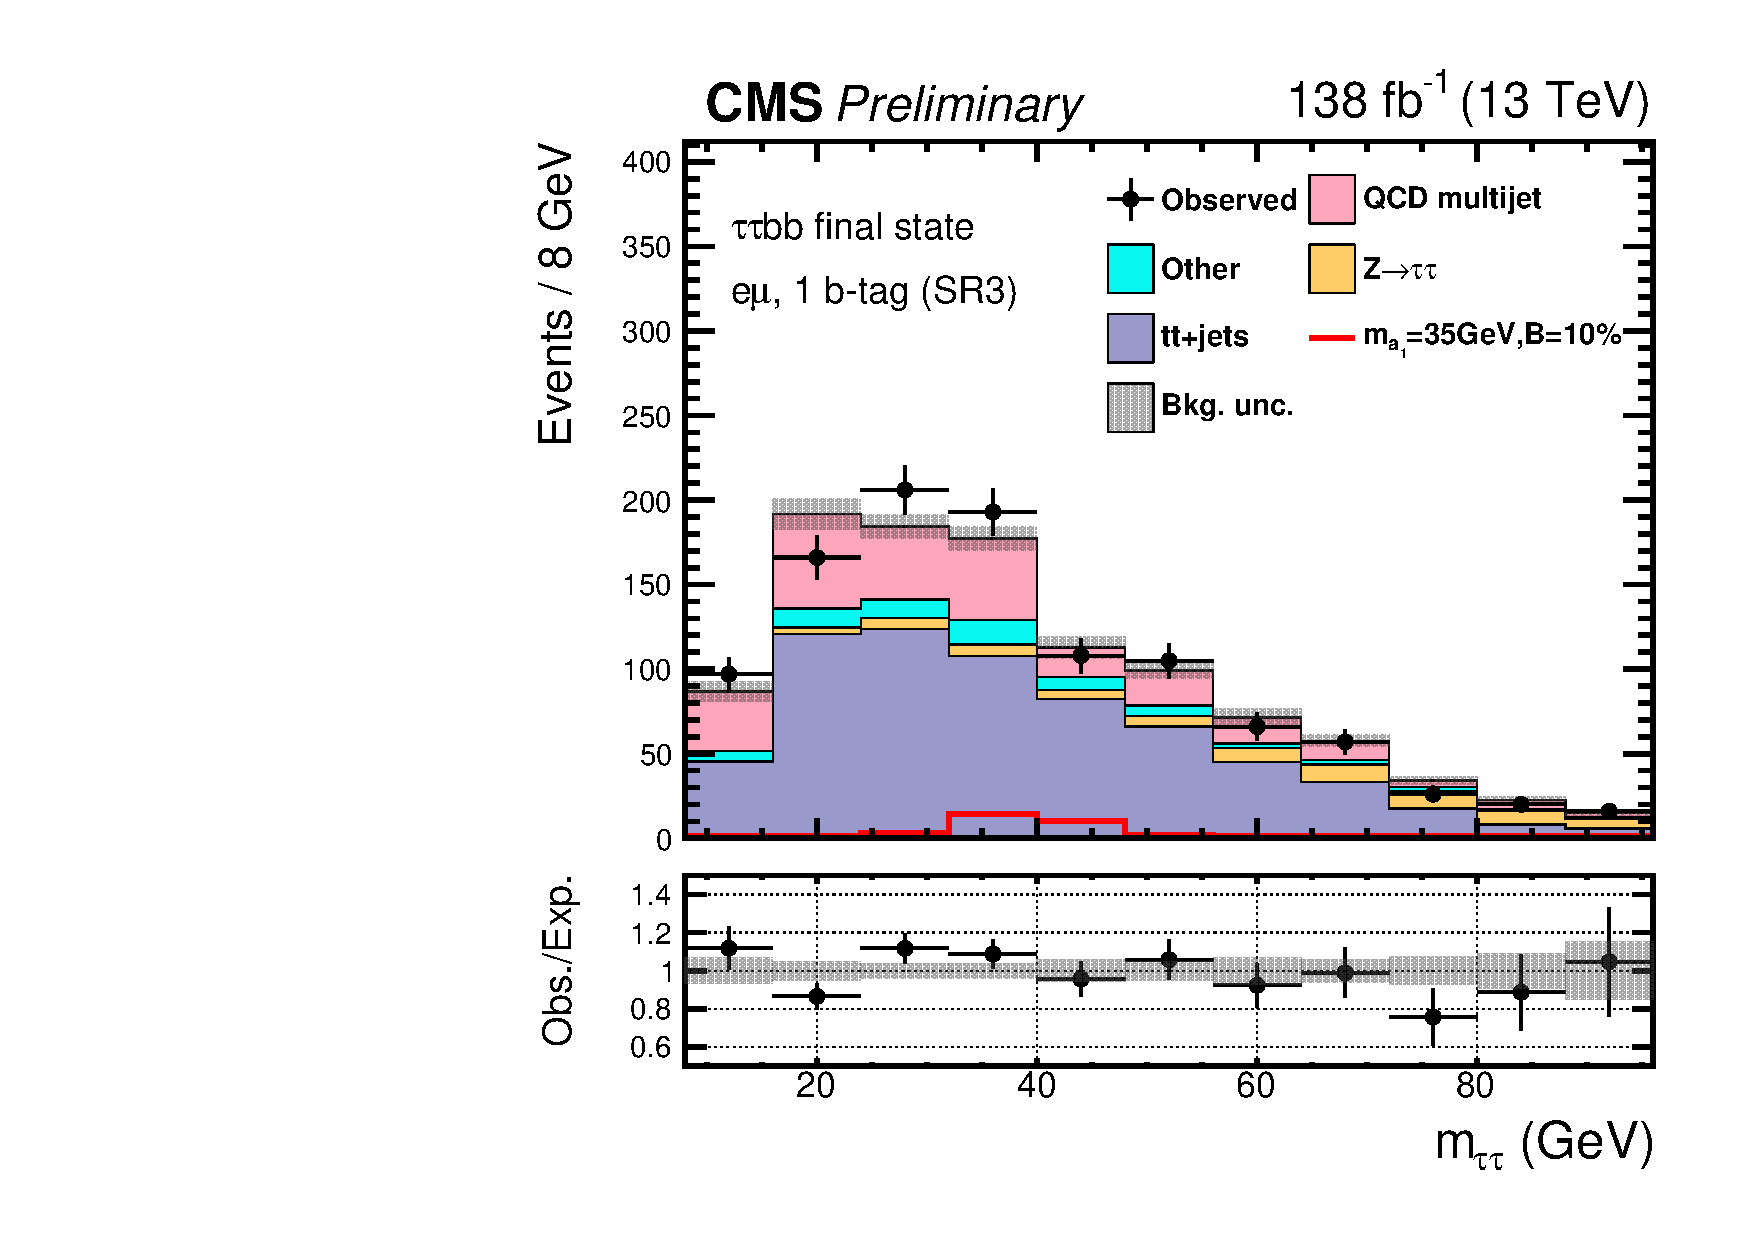
\includegraphics[width=0.32\textwidth]{figures/ch-13-results/em_all_3_post_prelim-yes.pdf}\\
        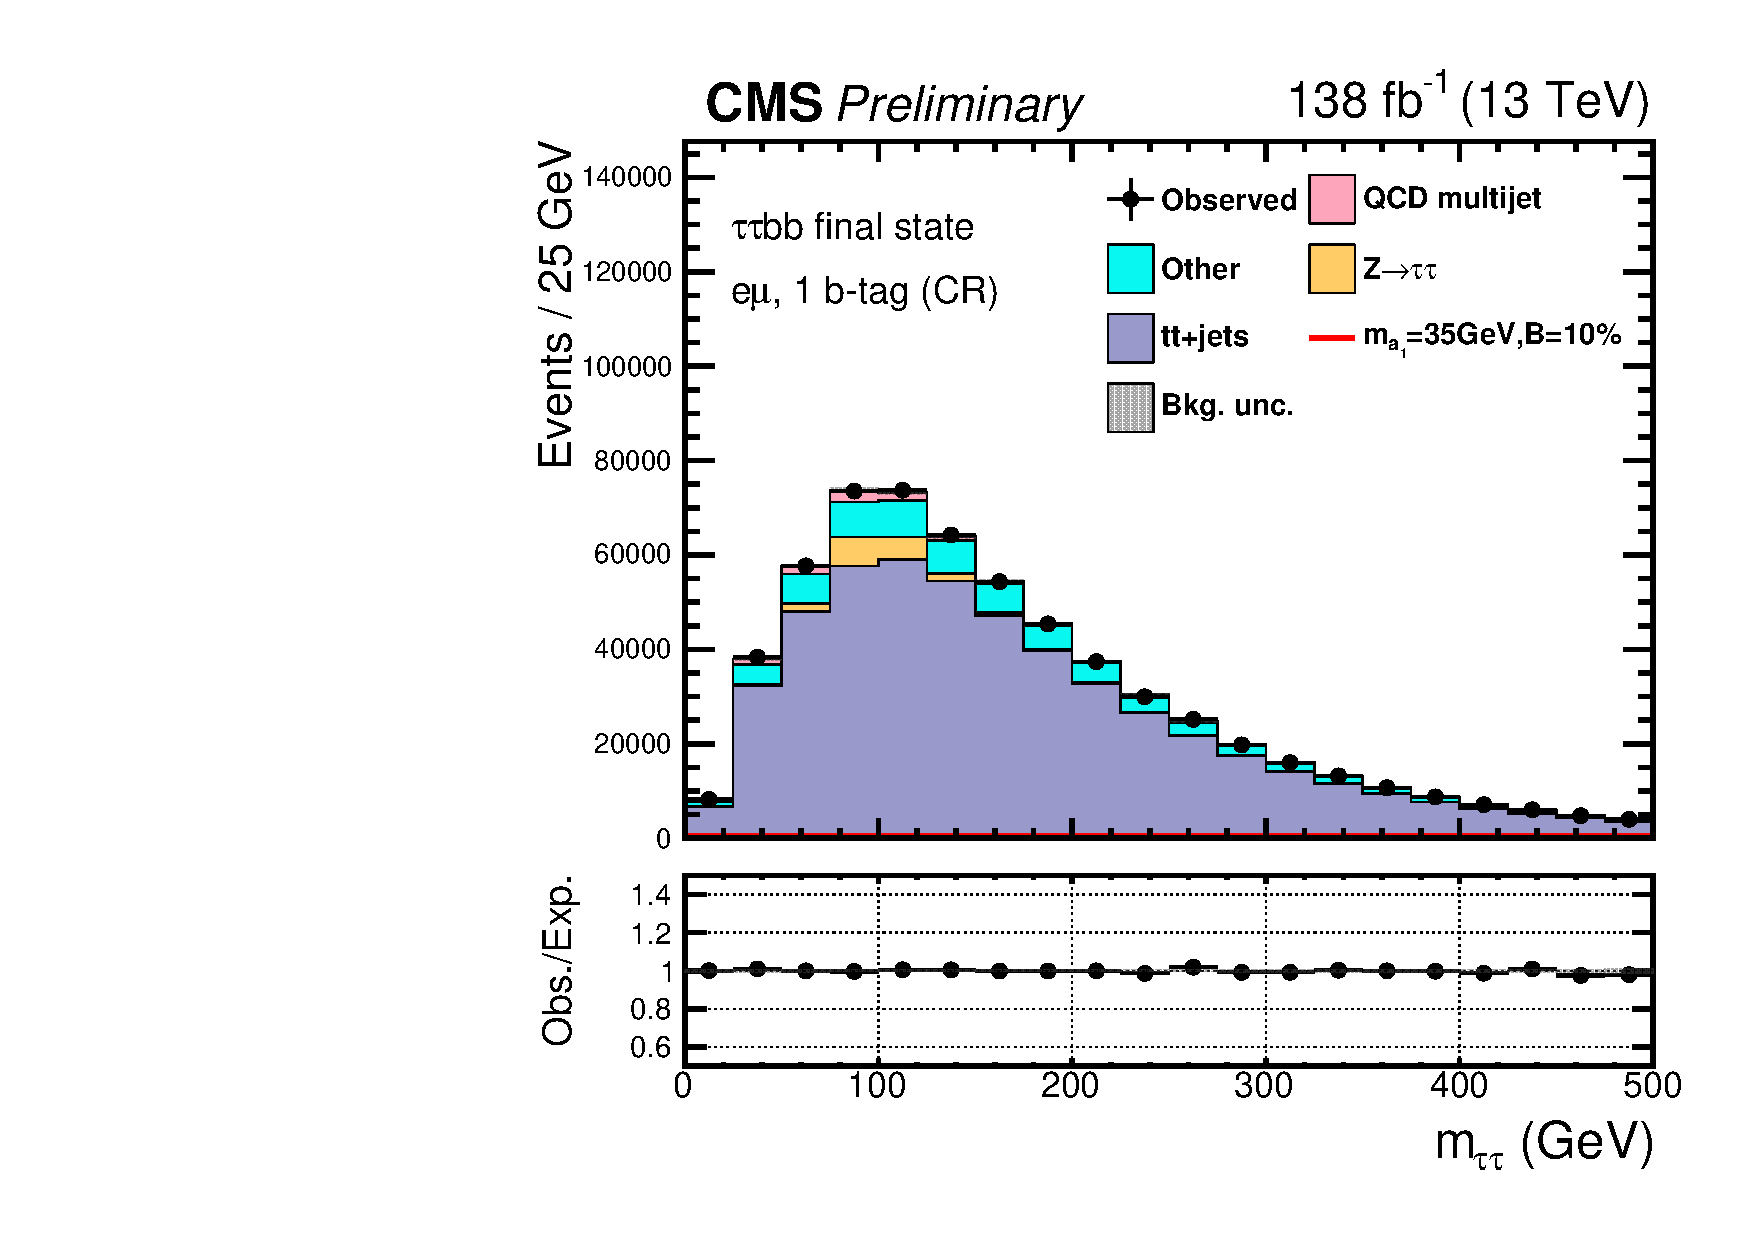
\includegraphics[width=0.32\textwidth]{figures/ch-13-results/em_all_4_post_prelim-yes.pdf}
        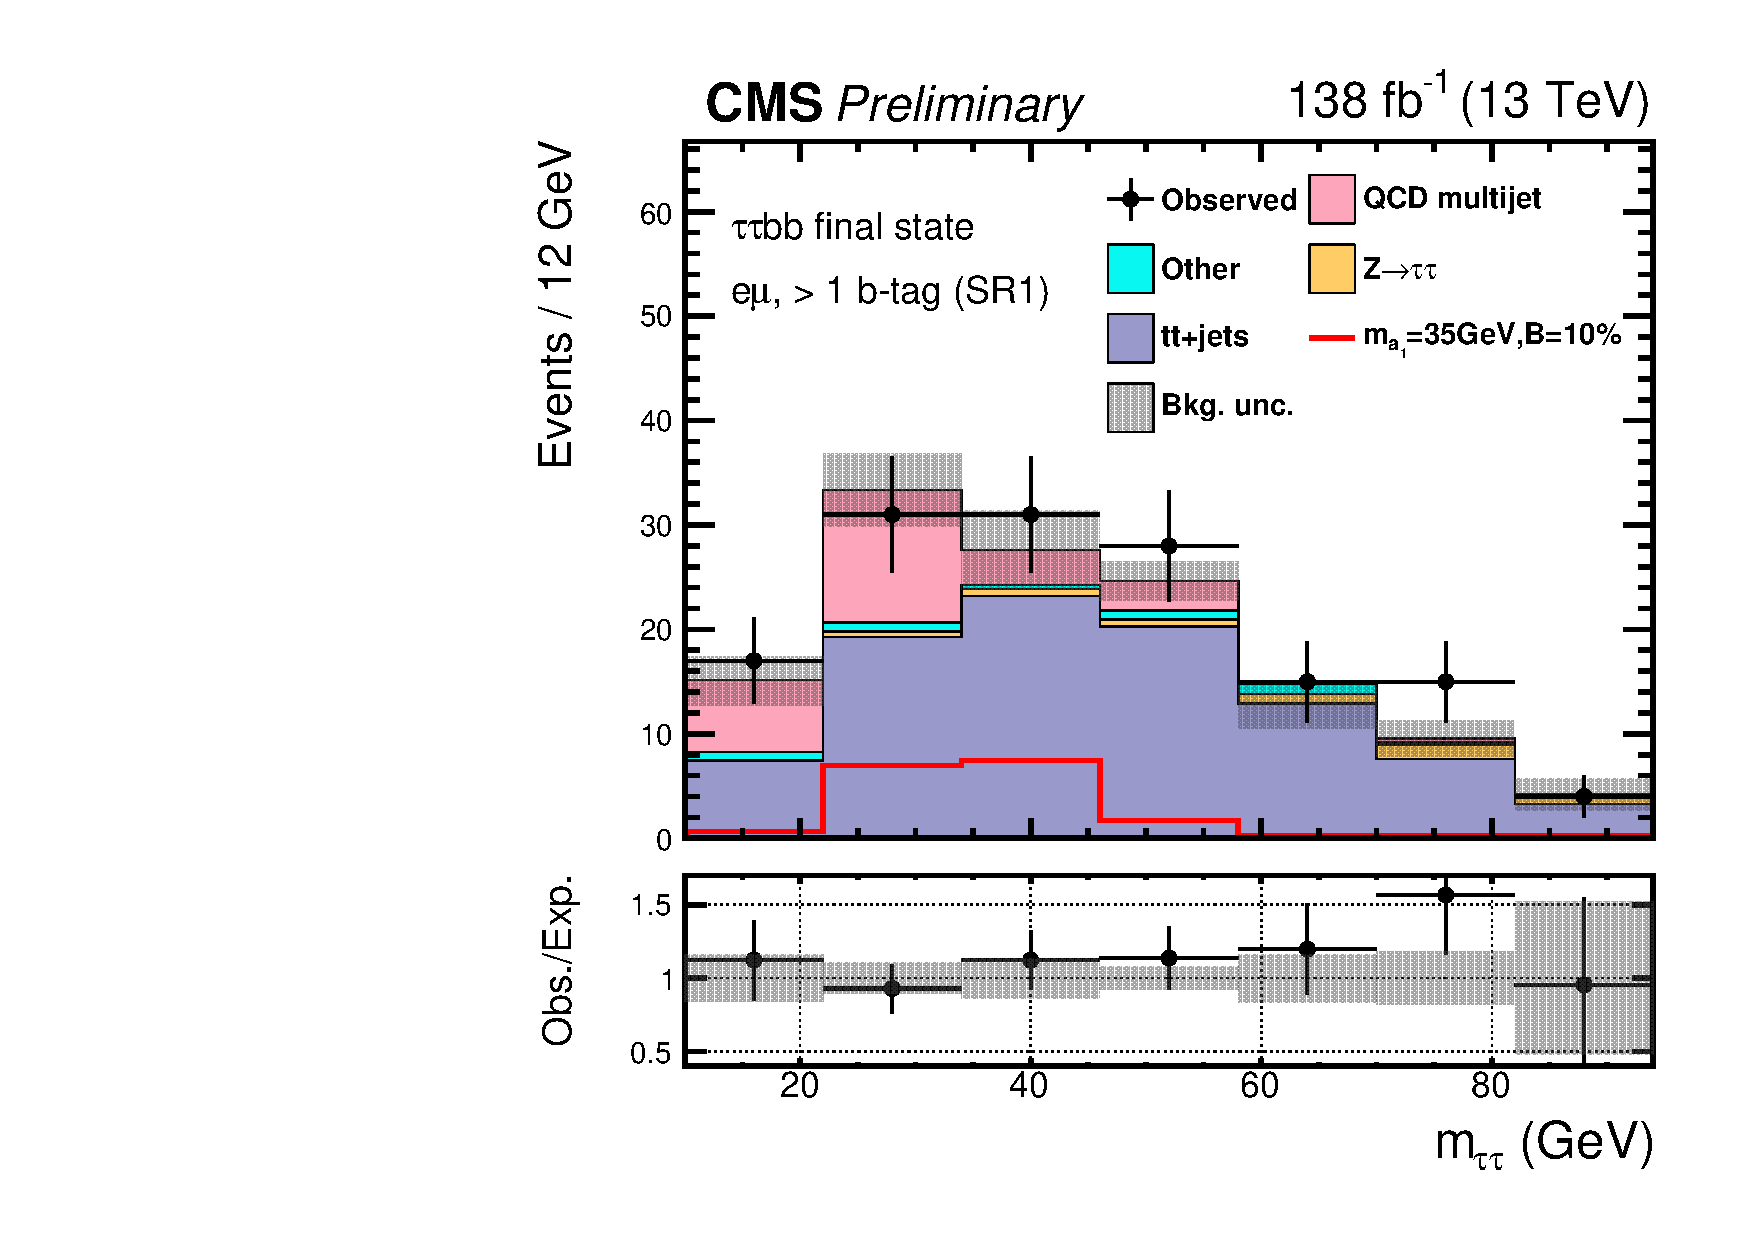
\includegraphics[width=0.32\textwidth]{figures/ch-13-results/em_all_5_post_prelim-yes.pdf}
        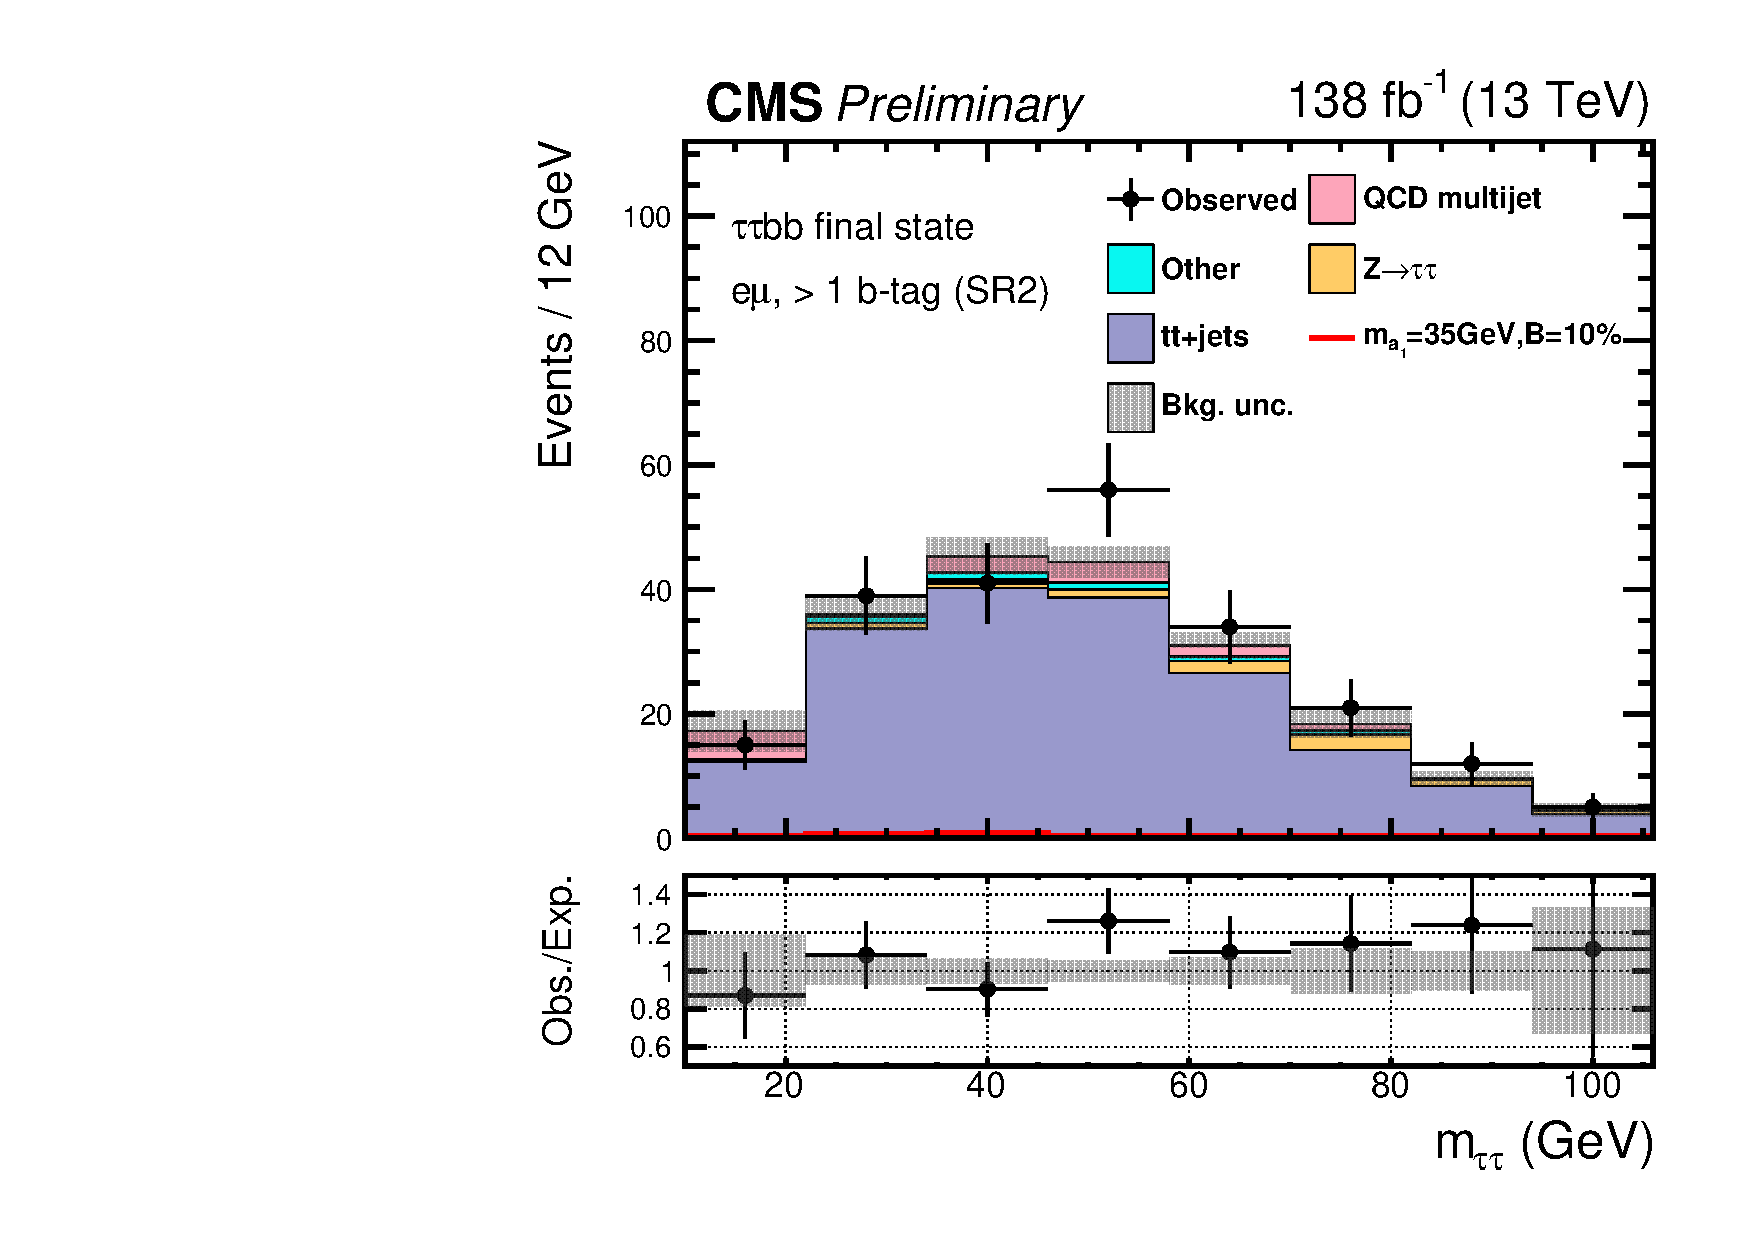
\includegraphics[width=0.32\textwidth]{figures/ch-13-results/em_all_6_post_prelim-yes.pdf}\\
        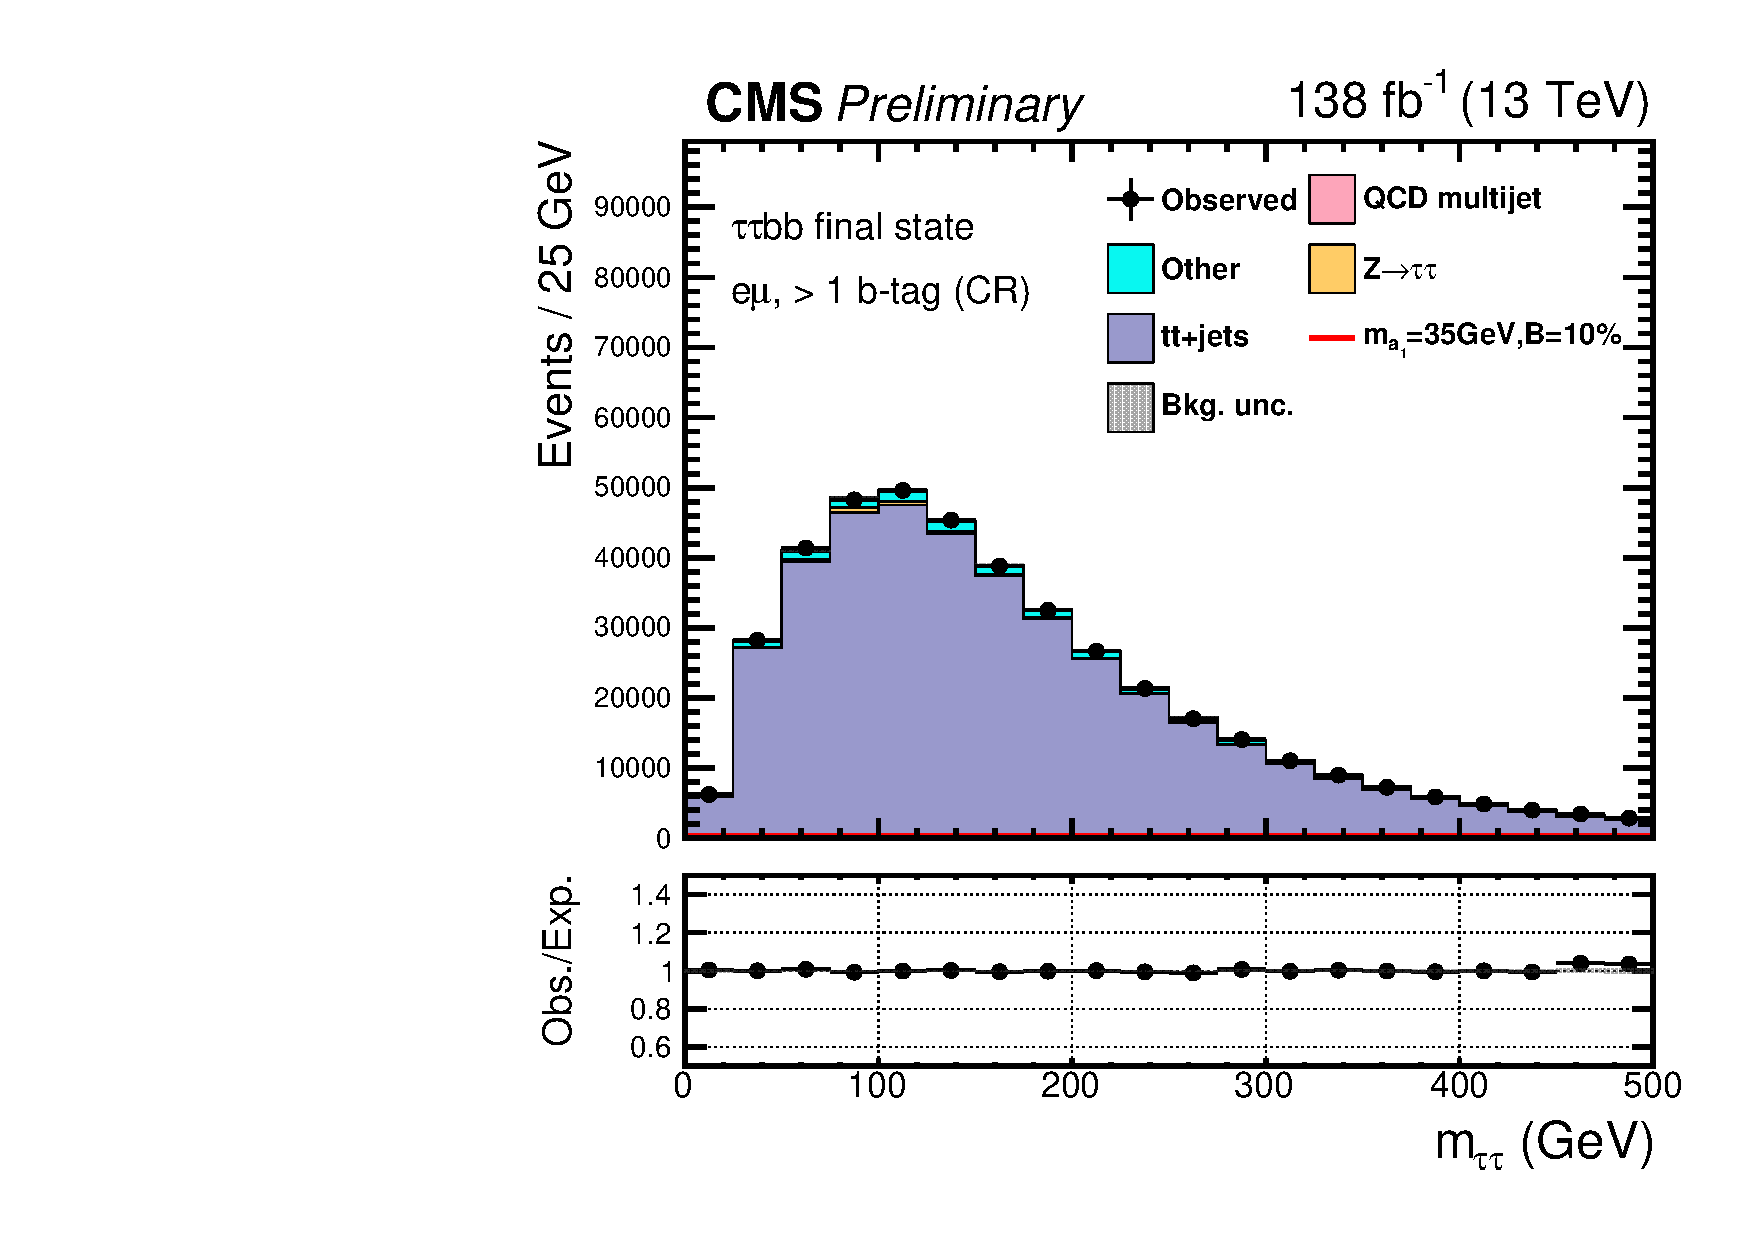
\includegraphics[width=0.32\textwidth]{figures/ch-13-results/em_all_7_post_prelim-yes.pdf}
    \end{center}
    \caption[Postfit final $m_{\tau\tau}$ distributions in the $e\mu$ channel.]{Postfit final $m_{\tau\tau}$ distributions in the $e\mu$ channel \cite{CMS-AN-20-213}. Statistical and systematic uncertainties are included. \textit{Top row:} 1 b-tag jet categories: three signal regions (SR1, SR2, and SR3). \textit{Middle row, left to right:} 1 b-tag jet categories: control region (CR), and 2 b-tag jet categories: signal regions (SR1 and SR2). \textit{Bottom:} 2 b-tag jet categories: control region (CR).}
    \label{fig:results_mtt_postfit_emall}
\end{figure}


The 95\% CL exclusion limits on the signal strength of the branching ratio $\mathcal{B}(h \rightarrow aa \rightarrow bb\tau\tau)$, shown in percentage and normalized to the Standard Model Higgs production cross-section, is shown in Fig. \ref{fig:results_limits}. The pseudoscalar mass hypotheses $m_a$ between 15 GeV and 60 GeV are searched for in all channels. The $e\mu$ channel is the only channel that can provide sensitivity to the $m_a = 12$ GeV mass point, as its cut on the $\Delta R$ between the two $\tau$ legs is the smallest, which increases the signal acceptance for low mass signals.

Combined expected (observed) limits between 1.4 and 5.6\% (1.7 and 7.6\%) are set for the pseudoscalar mass range between 12 and 60 GeV. The best sensitivity is attained at intermediate mass points, since the analysis targets a resolved signature: at low mass points, objects have a boosted signature, and at high mass points, the $m_{\tau\tau}$ distributions in signal have larger overlap with background distributions.

\begin{figure}[h!]
    \begin{center}
        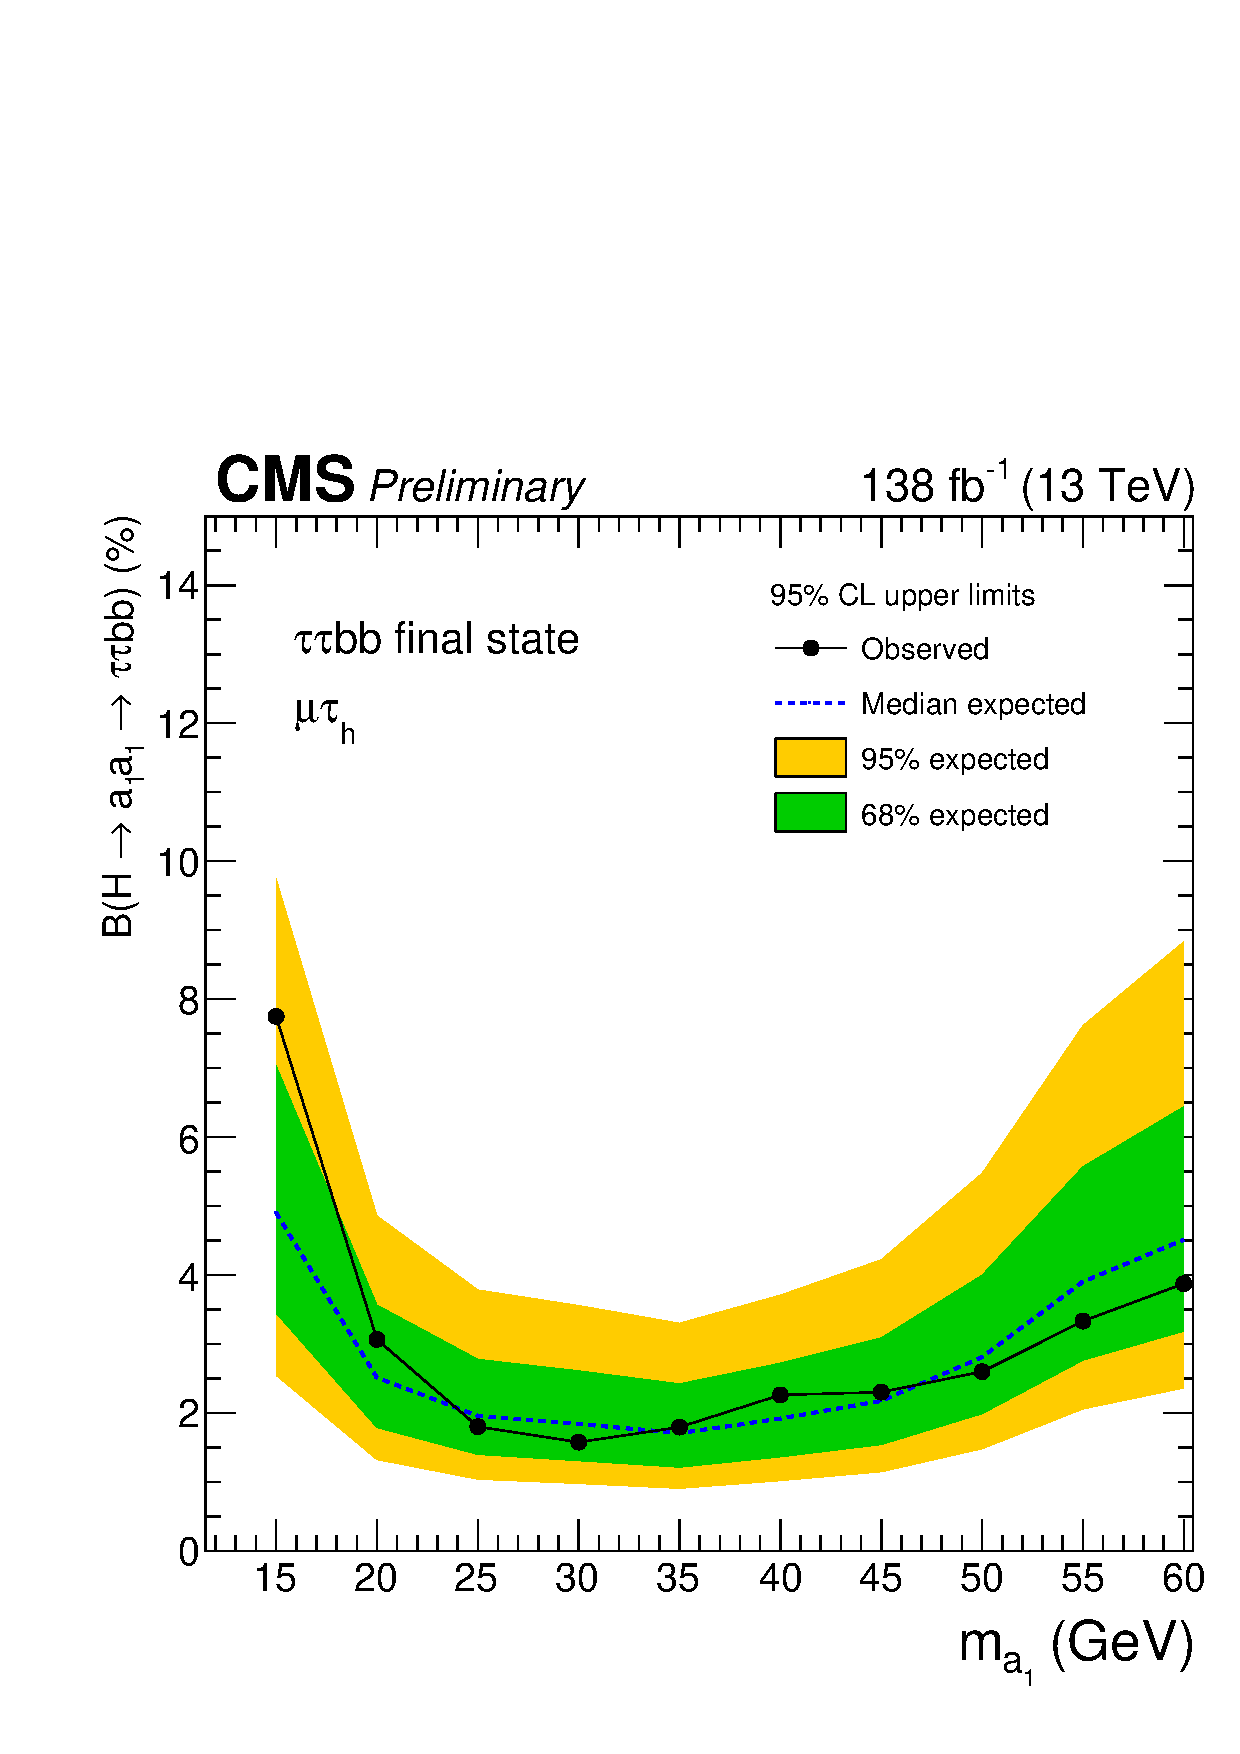
\includegraphics[width=0.45\textwidth]{figures/ch-13-results/Limit_mt_prelim.pdf}
        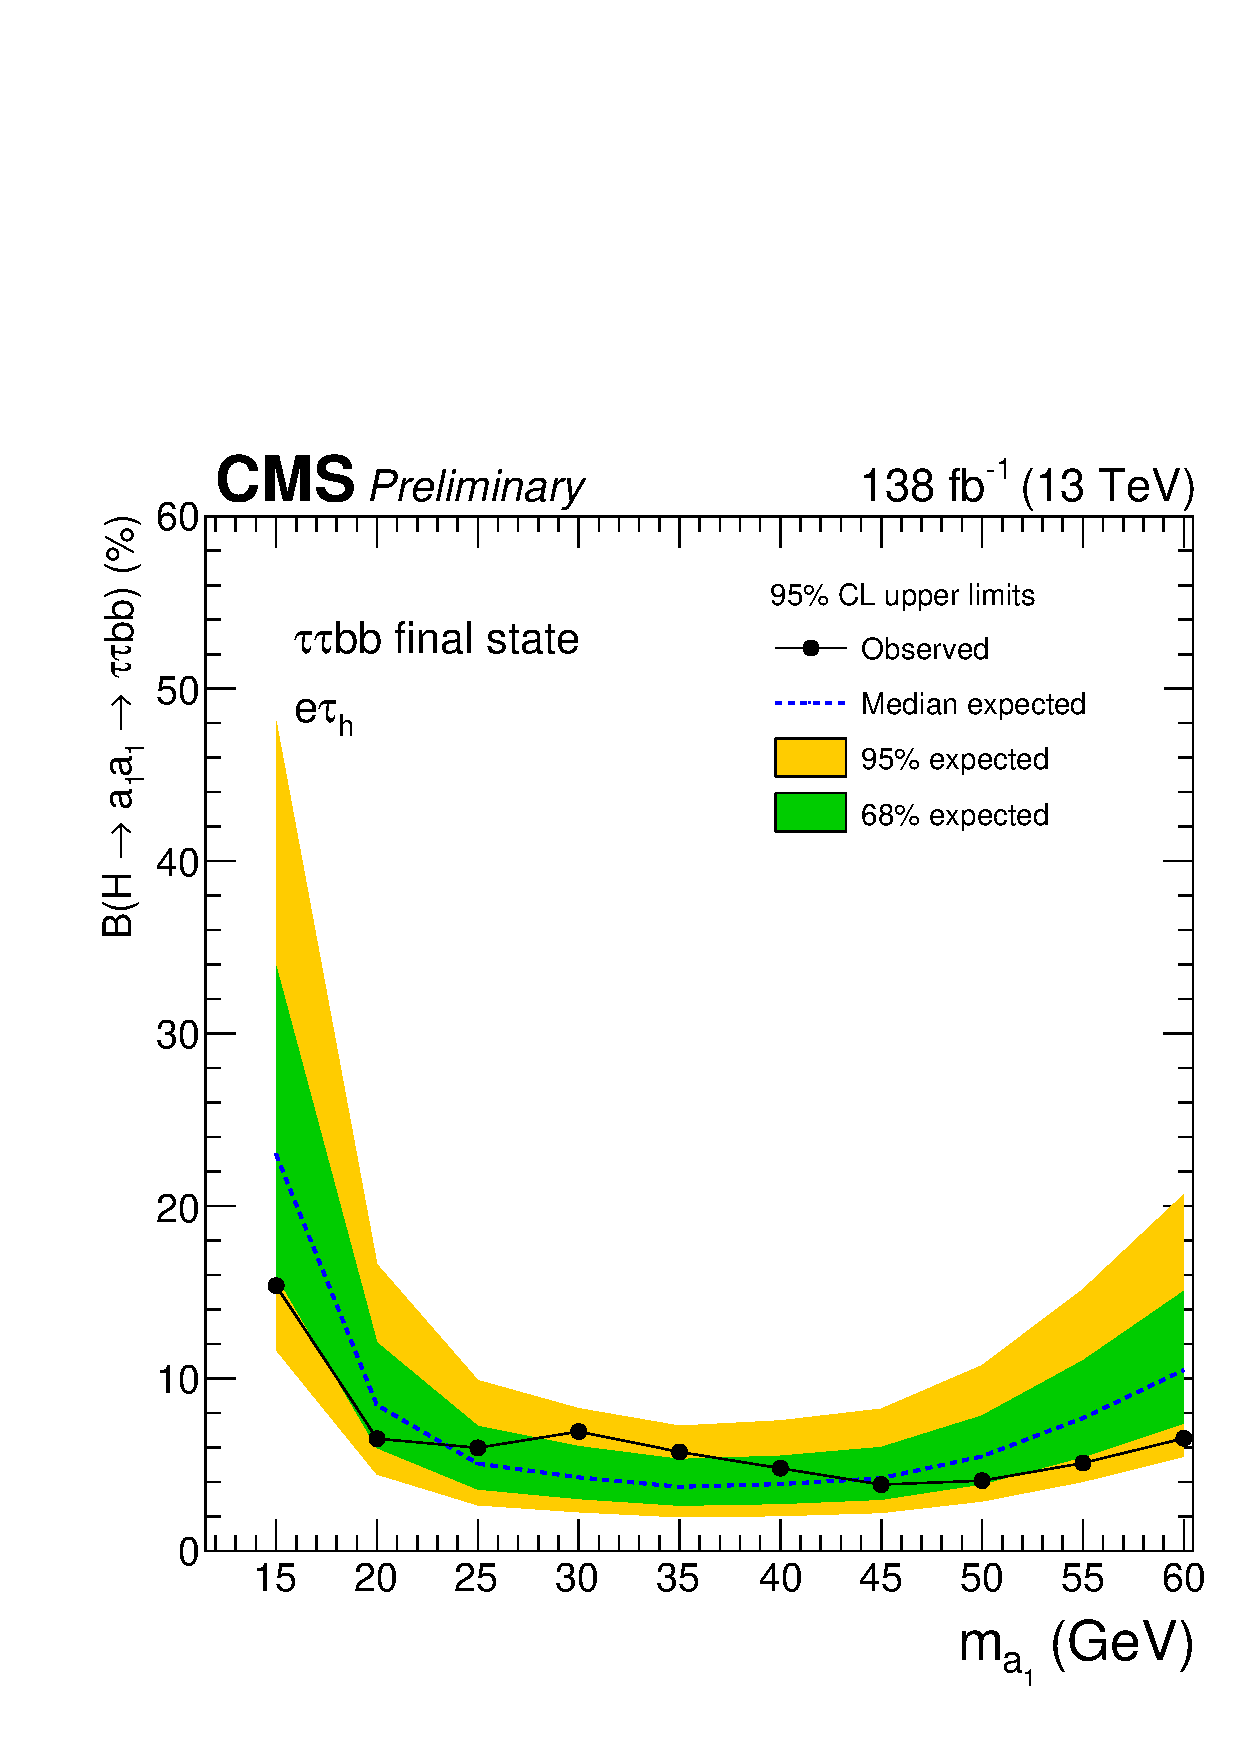
\includegraphics[width=0.45\textwidth]{figures/ch-13-results/Limit_et_prelim.pdf}\\
        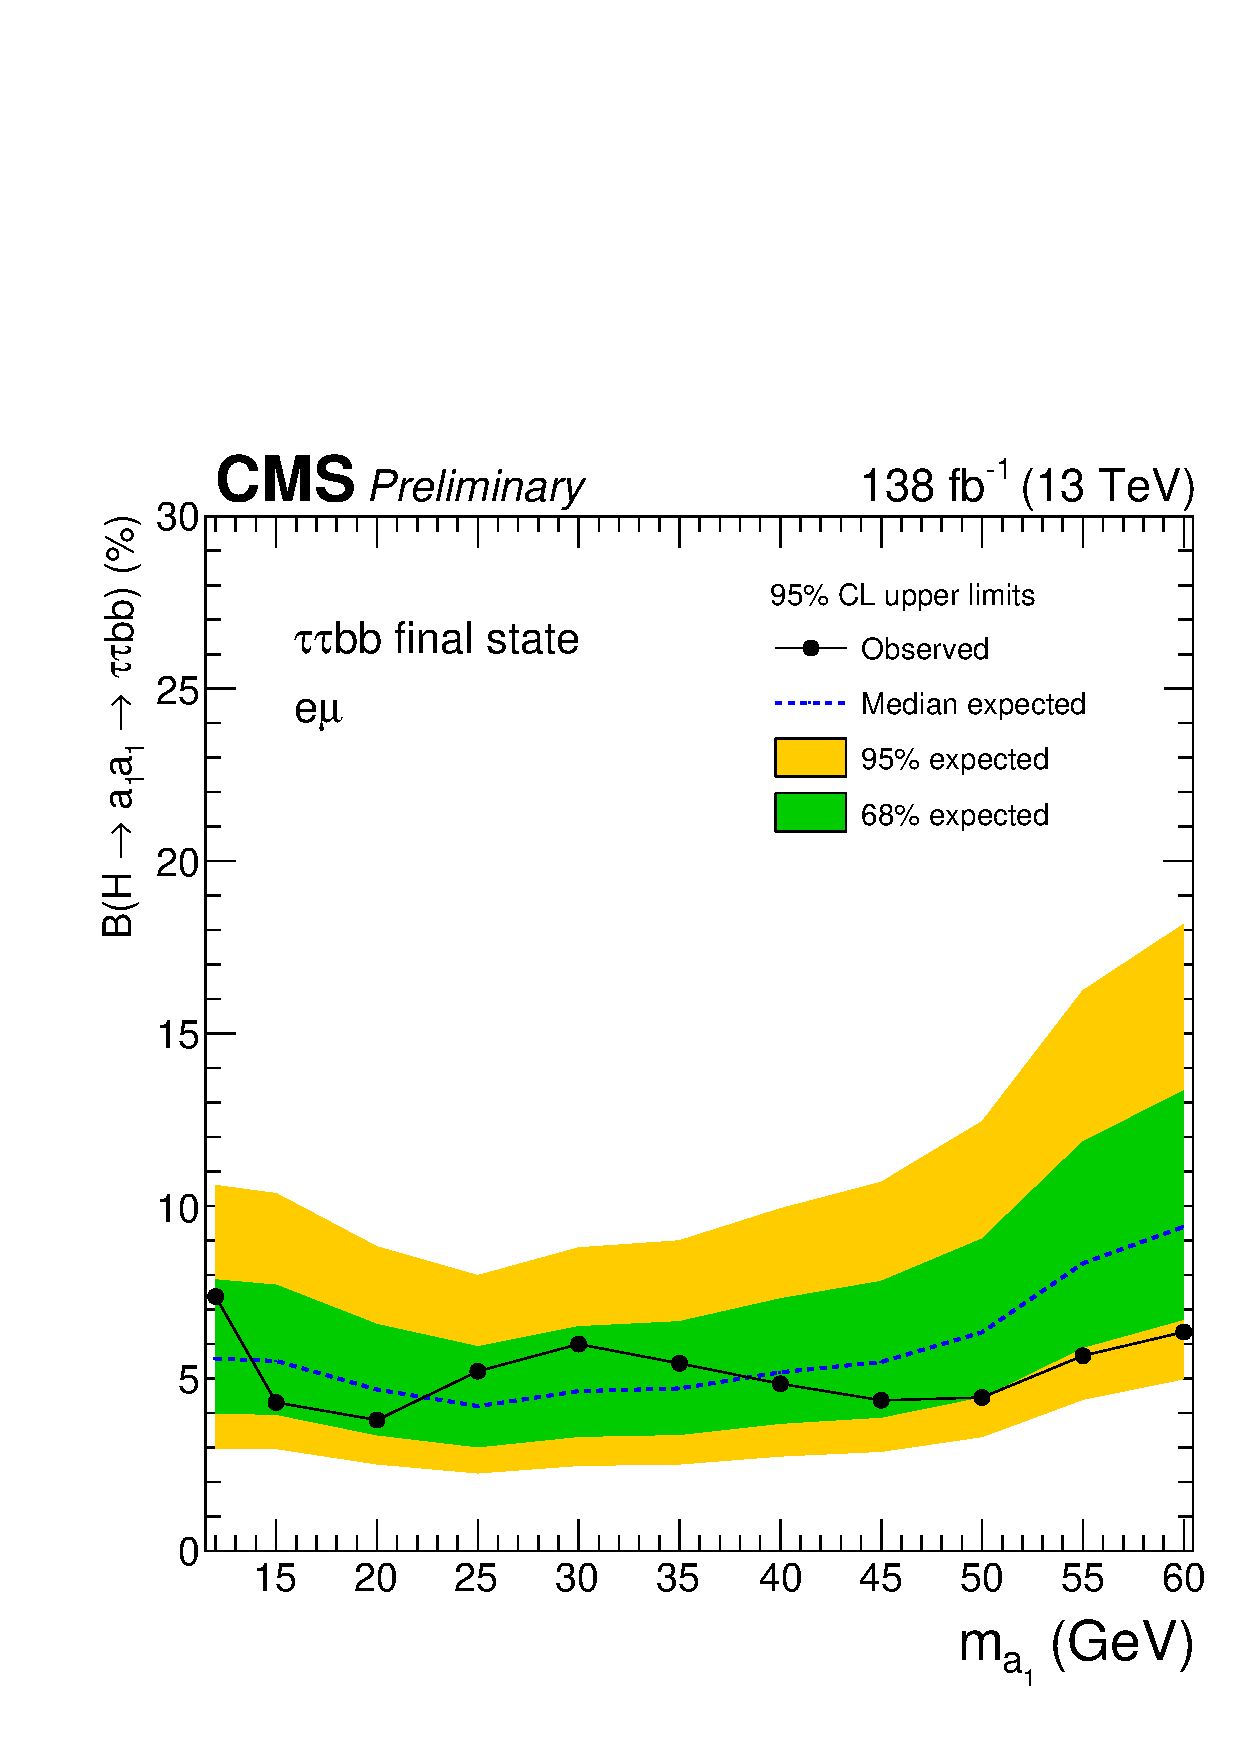
\includegraphics[width=0.45\textwidth]{figures/ch-13-results/Limit_em_prelim.pdf}
        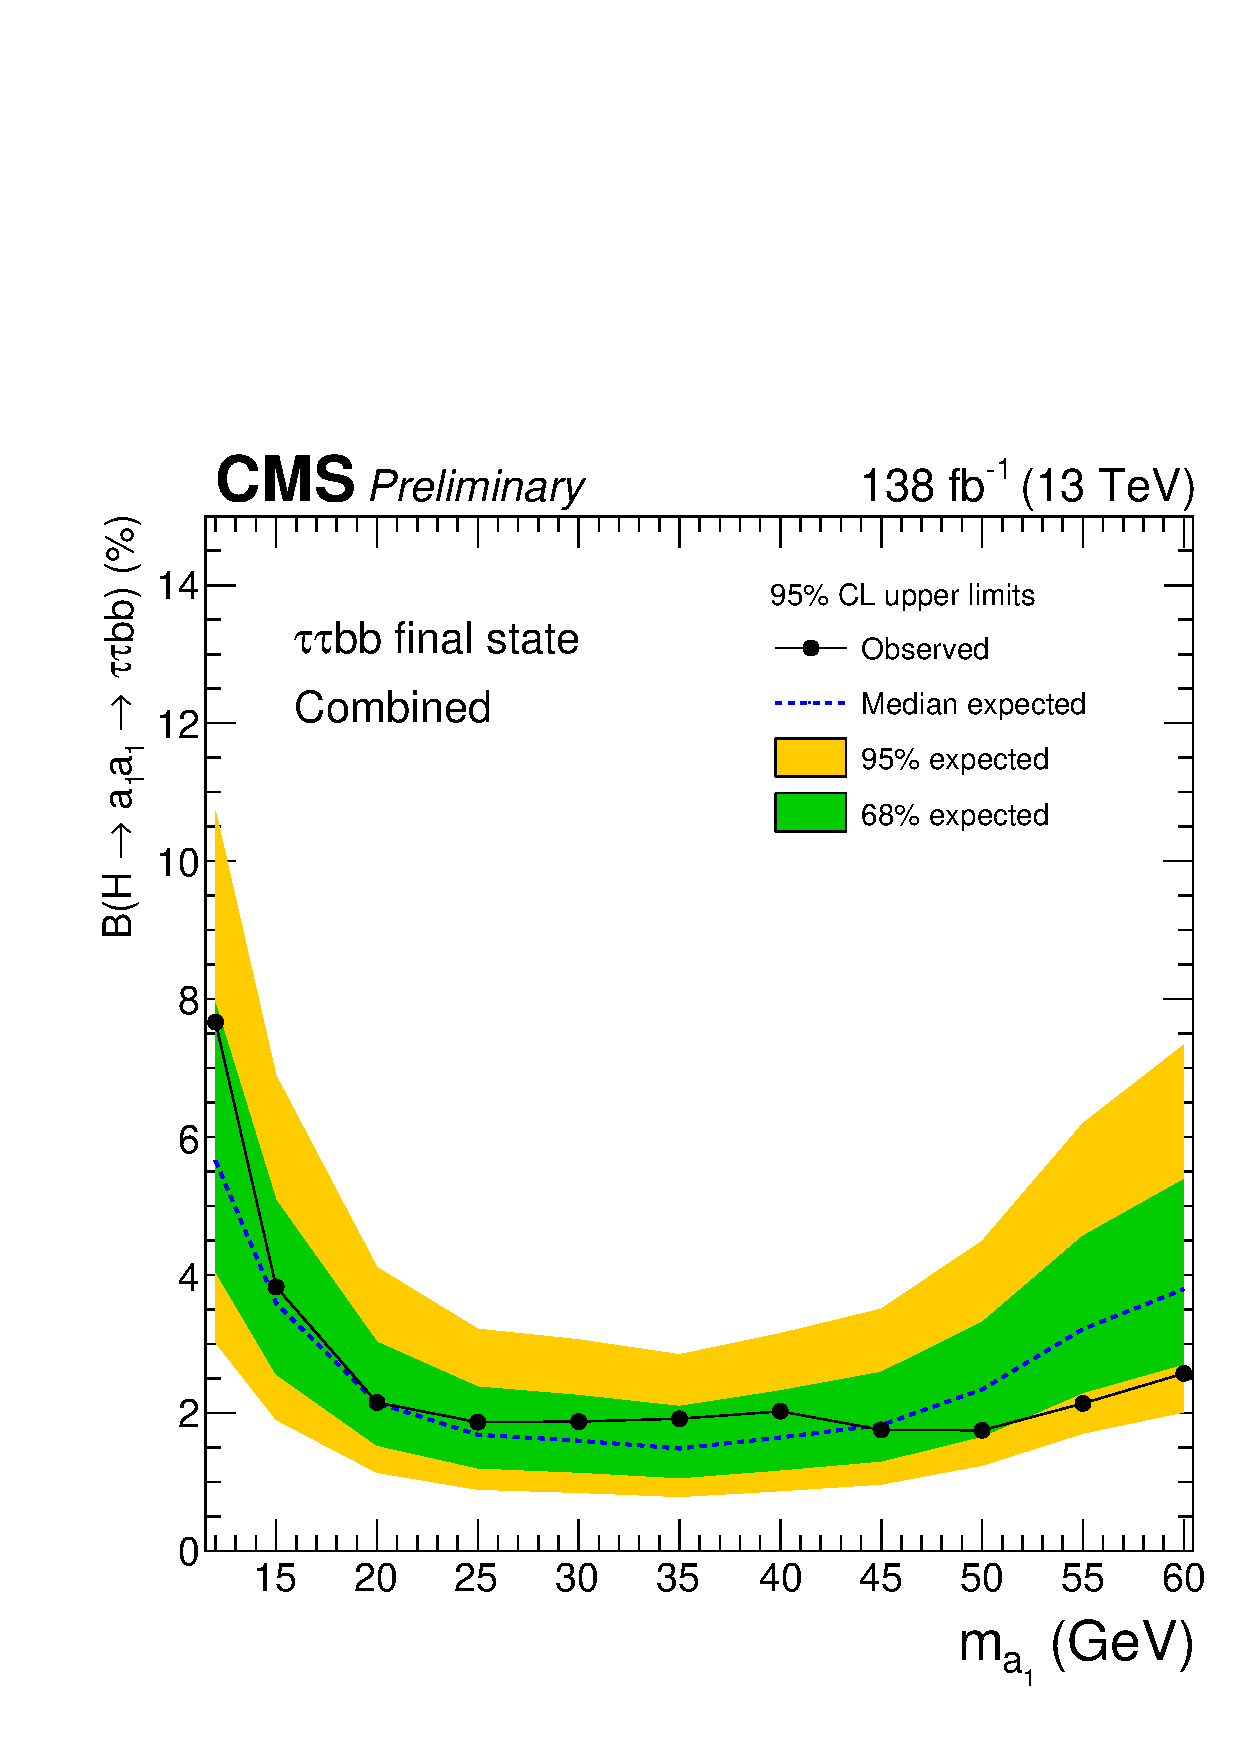
\includegraphics[width=0.45\textwidth]{figures/ch-13-results/Limit_all_prelim.pdf}
    \end{center}
    \caption[95\% CL exclusion limits on B($h\rightarrow aa\rightarrow bb\tau\tau$) in \%.]{95\% CL exclusion limits on B($h\rightarrow aa\rightarrow bb\tau\tau$) in \%, for the combination of all years by channel (\textit{top left}: $\mu\tau_{h}$ channel, \textit{top right:} $e\tau_{h}$ channel, and \textit{Bottom left:} $e\mu$ channel) and the combination of all channels (\textit{bottom right}) \cite{CMS-AN-20-213}.}
    \label{fig:results_limits}
\end{figure}



\section{Combination with $bb\mu\mu$ final state}
